\documentclass{article}

% The default option is the Main Track submission mode with double-blind reviewing.
\usepackage{neurips_2026}

\usepackage[utf8]{inputenc}
\usepackage[T1]{fontenc}
\usepackage{url}
\usepackage{booktabs}
\usepackage{microtype}
\usepackage{graphicx}
\usepackage{caption}
\usepackage{subcaption}
\usepackage{arydshln}
\usepackage{multirow}
\usepackage{rotating}
\usepackage{siunitx}
\usepackage{makecell}
\usepackage{bm}
\usepackage{amsmath}
\usepackage{amssymb}
\usepackage{mathtools}
\usepackage{amsthm}
\usepackage{gensymb}
\usepackage{enumitem}
\usepackage{algorithm}
\usepackage{algorithmic}
\usepackage{xcolor}
\usepackage{colortbl}
\usepackage{hyperref}
\usepackage{xspace}
\usepackage[capitalize,noabbrev]{cleveref}

\newcommand{\return}{\textbf{return }}
\newcommand{\Comment}[1]{\hfill $\triangleright$ #1}

\makeatletter
\DeclareRobustCommand\onedot{\futurelet\@let@token\@onedot}
\def\@onedot{\ifx\@let@token.\else.\null\fi\xspace}
\def\eg{\emph{e.g}\onedot} \def\Eg{\emph{E.g}\onedot}
\def\ie{\emph{i.e}\onedot} \def\Ie{\emph{I.e}\onedot}
\def\cf{\emph{c.f}\onedot} \def\Cf{\emph{C.f}\onedot}
\def\etc{\emph{etc}\onedot} \def\vs{\emph{vs}\onedot}
\def\wrt{w.r.t\onedot} \def\dof{d.o.f\onedot}
\def\aka{\emph{a.k.a}\onedot}
\def\etal{\emph{et al}\onedot}
\makeatother

\newcommand{\beginsupplement}{%
\setcounter{table}{0}
\renewcommand{\thetable}{S\arabic{table}}%
\setcounter{figure}{0}
\renewcommand{\thefigure}{S\arabic{figure}}%
}

\newcommand{\dgs}{\textit{d}GS\xspace}
\newcommand{\dbs}{\textit{d}BS\xspace}
\newcommand{\dgso}{\textit{d}GS-O\xspace}
\newcommand{\dfamily}{\textit{d}-splatting\xspace}
\newcommand{\modelname}{\dfamily}

\newcommand{\spacedcdashline}[1]{\noalign{\vspace{2pt}}\cdashline{#1}\noalign{\vspace{3pt}}}

\theoremstyle{plain}
\newtheorem{theorem}{Theorem}[section]
\newtheorem{proposition}[theorem]{Proposition}
\newtheorem{lemma}[theorem]{Lemma}
\newtheorem{corollary}[theorem]{Corollary}
\theoremstyle{definition}
\newtheorem{definition}[theorem]{Definition}
\newtheorem{assumption}[theorem]{Assumption}
\theoremstyle{remark}
\newtheorem{remark}[theorem]{Remark}

\title{Direct Conditional Parameterization for N-Dimensional Splatting}

\author{%
  Anonymous Author(s) \\
  Affiliation \\
  Address \\
  \texttt{email}
}

\begin{document}

\maketitle

\vspace{-1.5em}
\begin{center}
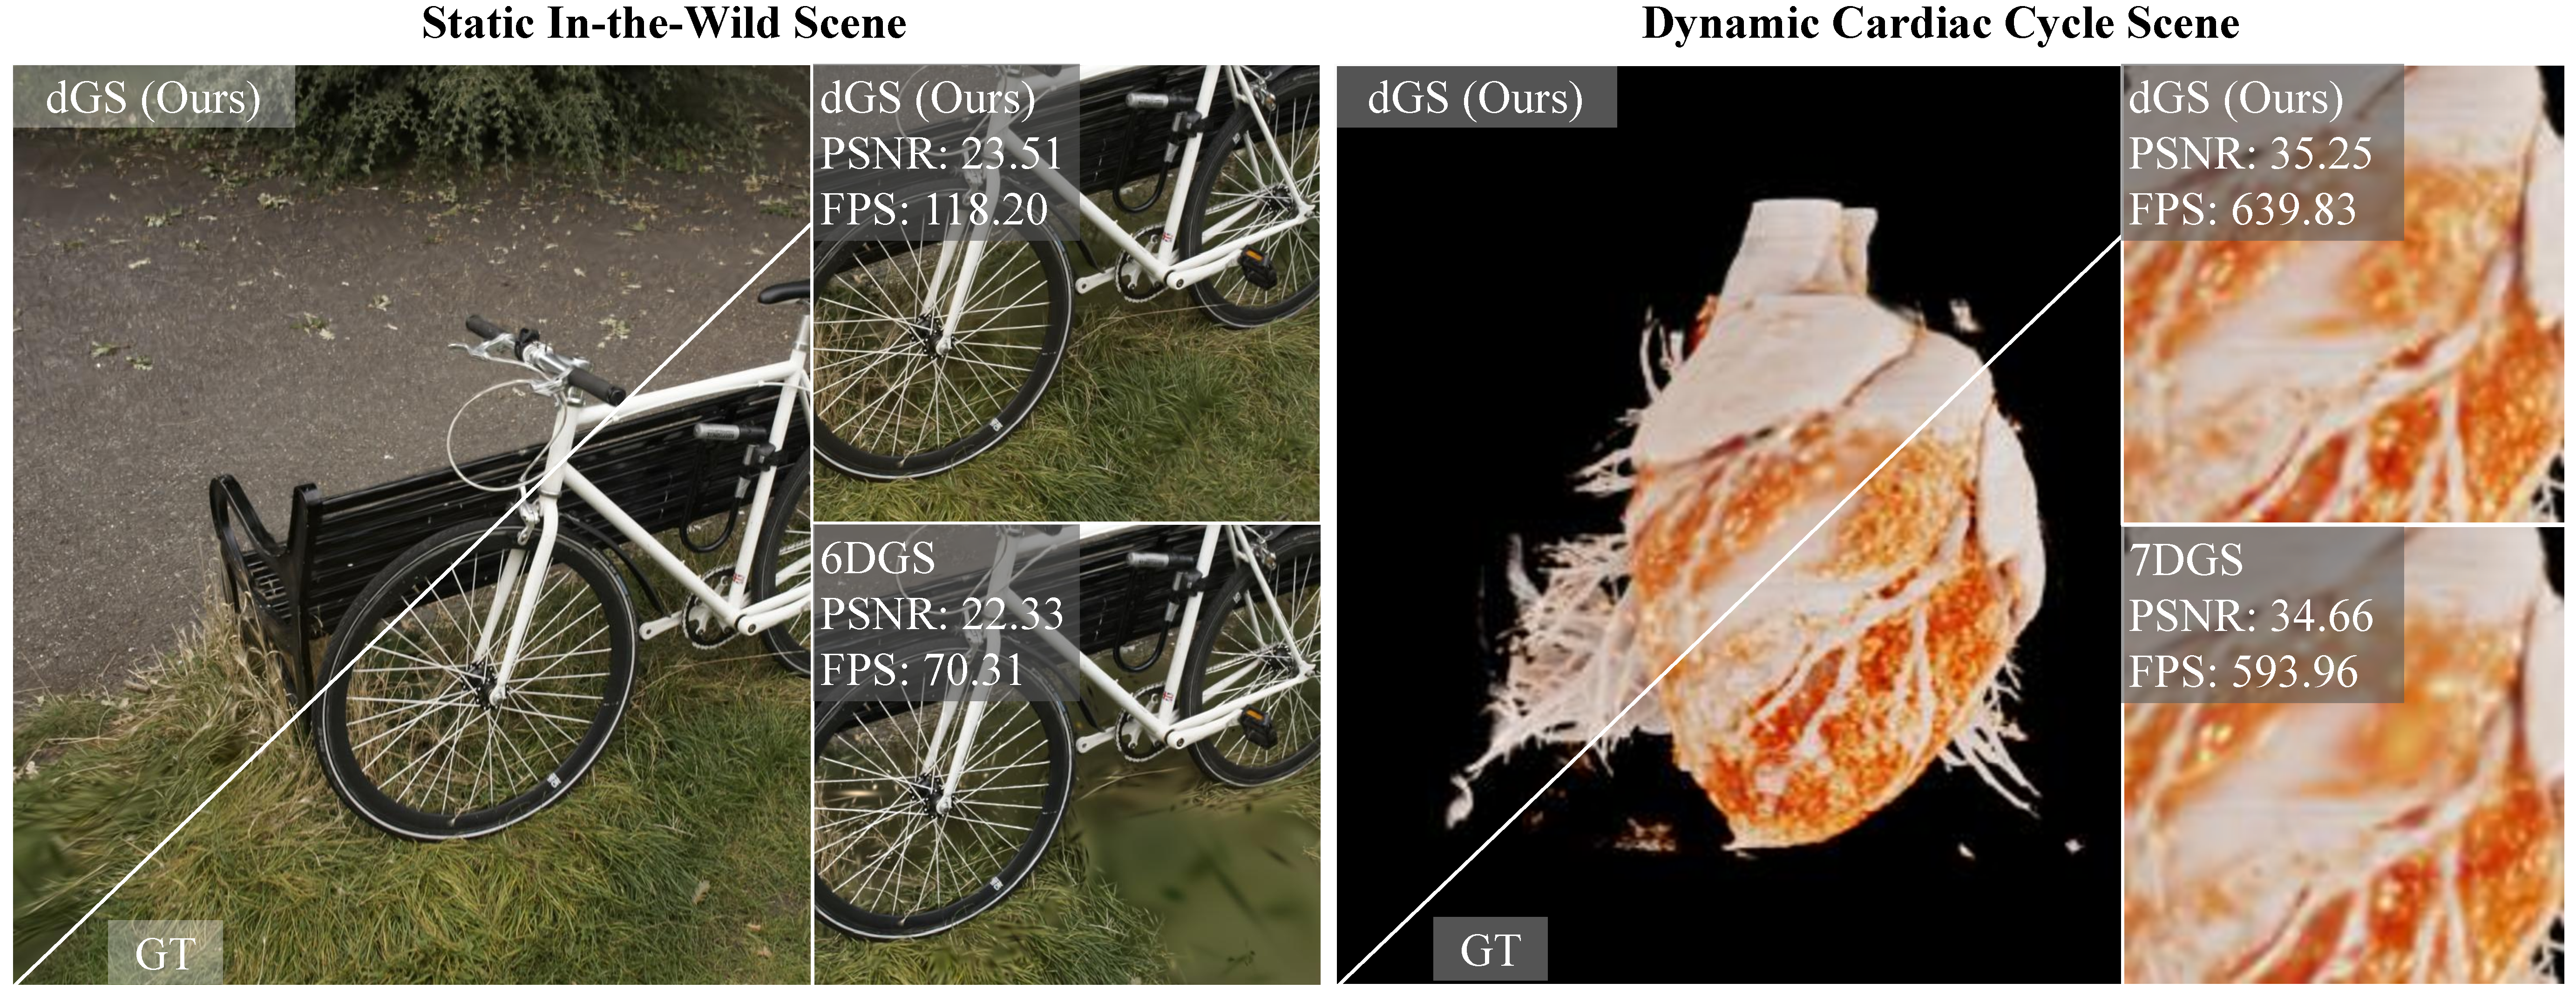
\includegraphics[width=0.95\linewidth]{figures/teaser.pdf}
\captionsetup{type=figure}
\captionof{figure}{\textbf{Rendering quality and efficiency comparison.} Our direct conditional parameterization yields two methods: \dgs{} (Gaussian kernel) outperforms its implicit-conditioning counterpart 6DGS \citep{gao20246dgs} on the static \texttt{bicycle} scene (left), and \dbs{} (Beta kernel) outperforms UBS \citep{liu2025universal} on the dynamic \texttt{heart1} scene (right). Both achieve higher quality and higher efficiency than their covariance-derived predecessors.}
\label{fig:teaser}
\end{center}
\vspace{-0.5em}

\begin{abstract}
   N-dimensional splatting extends 3D Gaussian Splatting with conditioning variables such as view direction and time to model view-dependent and dynamic effects. Each primitive is lifted into a joint distribution over 3D position and conditioning variables, and at render time is \emph{conditionally sliced} at the query to recover a 3D primitive whose mean, opacity, and covariance vary continuously with view or time. State-of-the-art methods span two kernel families, Gaussian (N-DGS, covering 6DGS and 7DGS) and Beta (UBS), but share the same conditional-slicing step: all three effects are derived from the joint covariance matrix per primitive in every forward pass, requiring matrix inversions and regression-matrix multiplications that scale with primitive count. The conditional-slicing step is kernel-agnostic, so a single improvement carries across families. We introduce direct conditional parameterization, replacing the covariance-derived form with explicit per-effect parameters: a Cholesky precision factor for opacity and a displacement matrix with learnable per-dimension coupling for position. Applied to both kernels, the parameterization yields \dgs{} (Gaussian) and \dbs{} (Beta). Across five static and dynamic benchmarks, \dgs{} and \dbs{} match or exceed their covariance-derived counterparts on quality (up to +0.97 dB on Mip-NeRF 360) while running 6.9--10.8$\times$ faster at the slicing step and up to 2.66$\times$ faster end-to-end. Direct conditioning is a kernel-agnostic drop-in replacement for covariance-derived conditioning in N-dimensional splatting.
\end{abstract}


\section{Introduction}
\label{sec:introduction}
3D Gaussian Splatting (3DGS)~\citep{3dgs} achieves photorealistic novel-view synthesis at real-time speeds through explicit 3D Gaussian primitives. Real-world scenes, however, exhibit phenomena that static primitives cannot capture: specular reflections, temporal dynamics, and view-dependent geometry.

Recent work extends 3DGS along two largely orthogonal axes. The first is \textit{kernel shape}: alternatives to the Gaussian kernel include Beta kernels~\citep{liu2025deformable,liu2025universal}, generalized exponentials~\citep{hamdi2024gesgeneralizedexponentialsplatting}, and Student-t distributions~\citep{zhu20253dstudentsplattingscooping}. The second is \textit{dimensionality}: N-dimensional Gaussians (N-DG)~\citep{diolatzis2024n}, refined as 6DGS~\citep{gao20246dgs} and 7DGS~\citep{gao20257dgs} (collectively N-DGS), lift each primitive into a joint distribution over 3D position and conditioning variables (view direction with $C{=}3$, view+time with $C{=}4$). At render time, the $(3{+}C)$-dimensional primitive is \textit{conditionally sliced} at the current query (a view direction or timestamp) using the conditional Gaussian formulas: the mean shifts, the opacity is modulated by a kernel evaluated at the query, and the spatial covariance receives a correction term. Universal Beta Splatting (UBS)~\citep{liu2025universal} combines the two axes by replacing the Gaussian opacity decay with an anisotropic Beta kernel while inheriting the same conditional-slicing structure. N-DGS and UBS together cover the state of the art in N-dimensional splatting.

Despite their different kernels, N-DGS and UBS share the same conditional-slicing step, and this is where the per-primitive cost concentrates. Read-out of the three effects requires inverting the query-block of the covariance, multiplying it against a regression matrix, and applying a covariance-correction product (Table~\ref{tab:comparison_overview}). These operations run once per primitive in every forward pass, so the total cost grows linearly with primitive count, which on large scenes like Mip-NeRF 360 reaches millions. The shared covariance structure also rigidly ties opacity and position coupling, since both effects are read out of the same matrix, and the conditioning is numerically fragile when the query-block becomes ill-conditioned.

\textbf{Our insight.} The covariance-derived form parameterizes more than the slicing step actually needs. Opacity decay only needs a precision matrix in the query space (so that the kernel can compute a distance from the query to the canonical view/time); position shift only needs a $3{\times}C$ displacement matrix scaled by the query deviation. Both can be parameterized \textit{directly} as small dense parameters per primitive, rather than read out of an inverted joint covariance. Doing so eliminates the implicit derivation cost, breaks the rigid coupling between position and opacity (each can carry its own learnable strength), and avoids the ill-conditioning risks of the joint covariance.

We introduce \textbf{direct conditional parameterization} for N-dimensional splatting. Opacity uses a directly parameterized Cholesky precision factor, and position uses a directly parameterized displacement matrix with learnable per-dimension coupling that decouples position from opacity by default and recovers full coupling on demand. Because the change touches only the conditioning step, the same parameterization is kernel-agnostic and carries across kernel families: we instantiate it as \dgs{} (Gaussian) for the direct counterpart of N-DGS and \dbs{} (Beta) for the direct counterpart of UBS. Pairing each direct method with its covariance-derived counterpart (\dgs{} vs.\ N-DGS, \dbs{} vs.\ UBS) isolates the contribution of direct conditioning from the choice of kernel.

Our contributions are:

\begin{itemize}[leftmargin=*]
\item \textbf{Direct conditional parameterization} for N-dimensional splatting: a kernel-agnostic alternative to covariance-derived conditioning that explicitly parameterizes opacity precision (via a Cholesky factor) and position displacement (via a spatially-scaled bounded matrix with learnable per-dimension coupling).

\item \textbf{Two kernel instantiations and matched-pair evaluation.} We develop the formulation for the Gaussian kernel (\dgs{}, the direct counterpart of N-DGS) and show that the same conditioning extends to the Beta kernel via a drop-in opacity substitution (\dbs{}, the direct counterpart of UBS). Pairing each direct method with its covariance-derived counterpart isolates the gain from direct conditioning from the choice of kernel.

\item \textbf{Efficient CUDA implementation.} Fused, register-level CUDA kernels for direct conditioning and for the N-DGS/UBS baselines, achieving 6.9--10.8$\times$ faster slicing than the covariance-derived baselines and up to 2.66$\times$ faster end-to-end rendering. The N-DGS baseline was previously only available as a PyTorch implementation; we provide a fair CUDA comparison.
\end{itemize}


\section{Related Work}
\label{sec:related_work}

\textbf{3D Gaussian Splatting.}
3D Gaussian Splatting (3DGS)~\citep{3dgs} achieves real-time novel view synthesis through explicit 3D Gaussian primitives with spherical harmonic color encoding, and has inspired a wide range of extensions to anti-aliasing~\citep{yu2023mipsplattingaliasfree3dgaussian,yan2024multiscale3dgaussiansplatting}, densification~\citep{kheradmand20243dgaussiansplattingmarkov}, compression~\cite{lee2024compact,morgenstern2024compact}, and semantic modeling~\cite{shi2023languageembedded3dgaussians,zhou2024feature3dgssupercharging3d}. The original formulation remains static, relying on spherical harmonics alone for view dependence and offering no mechanism for temporal dynamics or view-dependent geometry.

\textbf{Alternative Kernel Designs.}
Several works replace the 3D Gaussian kernel with alternatives for better geometric fidelity: generalized exponentials~\cite{hamdi2024gesgeneralizedexponentialsplatting}, truncated~\cite{liu2025tnt}, second-order~\cite{zhang2025quadratic}, half-Gaussian~\cite{li20253d}, and discontinuity-aware~\cite{qu2024disc} variants; Beta~\cite{liu2025deformable}, Student-t~\cite{zhu20253dstudentsplattingscooping}, and Gabor~\cite{zhou20253dgabsplat3dgaborsplatting} distributions; and non-volumetric primitives such as convex shapes~\cite{held20243dconvexsplattingradiance}, triangles~\cite{held2025triangle}, and radial kernels~\cite{huang2025deformable}. These works modify the 3D spatial kernel but do not address conditioning on view direction or time; the Beta kernel is later combined with N-D conditioning by UBS, discussed in the next paragraph.

\textbf{N-Dimensional Splatting.}
To model view-dependent and temporal effects, recent methods lift primitives into higher-dimensional spaces, conditioning on view direction or time alongside position. 4DGS~\cite{yang2023real} adds a temporal dimension for dynamic scene reconstruction, and N-DG~\cite{diolatzis2024n} establishes a general framework for arbitrary-dimensional Gaussians. 6DGS~\cite{gao20246dgs} jointly models spatial position and view direction; 7DGS~\cite{gao20257dgs} adds time as well; we refer to the two collectively as N-DGS. Universal Beta Splatting (UBS)~\citep{liu2025universal} extends the same paradigm to Beta kernels with per-dimension bandwidth control. N-DGS and UBS together cover the two kernel families currently used in N-dimensional splatting, and both inherit the covariance-derived conditioning step that our work replaces.

\textbf{Dynamic Scene Modeling.}
NeRF-based methods model dynamics through deformations: D-NeRF~\cite{pumarola2020dnerfneuralradiancefields} introduces canonical-to-deformed mappings, Nerfies~\cite{park2021nerfies} handles non-rigid motion, and HyperNeRF~\cite{park2021hypernerf} captures topological changes. For Gaussian Splatting, 4DGS~\cite{yang2023real} enables real-time dynamic rendering, Dynamic 3D Gaussians~\cite{luiten2023dynamic} combines canonical representations with learned deformations, and FreeTimeGS~\cite{wang2025freetimegs} allows Gaussians to appear at arbitrary times and locations with motion functions. These deformation-based approaches model dynamics as transformations of primitives, whereas N-dimensional splatting conditions a single primitive on temporal queries.


\section{Preliminary}

\paragraph{3D Gaussian Splatting}
3DGS~\cite{3dgs} represents a scene as a collection of anisotropic 3D Gaussians. Each primitive carries a mean $\boldsymbol{\mu}\in\mathbb{R}^3$, a covariance $\boldsymbol{\Sigma}\in\mathbb{R}^{3\times 3}$ factored as $\boldsymbol{\Sigma}=\mathbf{R}\mathbf{S}\mathbf{S}^\top\mathbf{R}^\top$ with rotation $\mathbf{R}$ (quaternion) and diagonal scale $\mathbf{S}=\operatorname{diag}(s_x,s_y,s_z)$, an opacity $\alpha\in[0,1]$, and view-dependent color via spherical harmonics. The representation is static: it has no mechanism for temporal dynamics or view-dependent geometry.

\paragraph{N-Dimensional Splatting}
To capture view-dependent and temporal effects, N-DGS~\cite{gao20246dgs,gao20257dgs} (Gaussian kernel) and UBS~\citep{liu2025universal} (Beta kernel) parameterize each primitive as a joint distribution over position $\mathbf{X}_p\in\mathbb{R}^3$ and query variables $\mathbf{X}_q\in\mathbb{R}^C$ (view direction for $C=3$, view+time for $C=4$):
\begin{align}
\begin{pmatrix} \mathbf{X}_p \\ \mathbf{X}_q \end{pmatrix} \sim \left(
\begin{pmatrix}
\boldsymbol{\mu}_p \\ \boldsymbol{\mu}_q
\end{pmatrix},
\begin{pmatrix}
\boldsymbol{\Sigma}_{pp} & \boldsymbol{\Sigma}_{pq} \\
\boldsymbol{\Sigma}_{pq}^\top & \boldsymbol{\Sigma}_{qq}
\end{pmatrix}
\right).
\end{align}
At query $\mathbf{q}$, both methods derive the conditional position, spatial covariance, and opacity from the same conditional Gaussian formulas:
\begin{align}
\boldsymbol{\mu}_{\text{cond}} &= \boldsymbol{\mu}_p + \boldsymbol{\Sigma}_{pq}\,\boldsymbol{\Sigma}_{qq}^{-1}(\mathbf{q}-\boldsymbol{\mu}_q), \label{eq:prelim_mu}\\
\boldsymbol{\Sigma}_{\text{cond}} &= \boldsymbol{\Sigma}_{pp} - \boldsymbol{\Sigma}_{pq}\,\boldsymbol{\Sigma}_{qq}^{-1}\,\boldsymbol{\Sigma}_{pq}^\top, \label{eq:prelim_sigma}\\
\alpha_{\text{cond}} &= \alpha \cdot \mathcal{K}\!\left(\mathbf{q}-\boldsymbol{\mu}_q;\,\boldsymbol{\Sigma}_{qq}\right). \label{eq:prelim_alpha}
\end{align}
$\mathcal{K}(\cdot;\boldsymbol{\Sigma}_{qq})$ is a kernel-specific opacity decay evaluated through the conditional precision $\boldsymbol{\Sigma}_{qq}^{-1}$. N-DGS uses a Gaussian kernel, $\mathcal{K}_{G}(\boldsymbol{\delta};\boldsymbol{\Sigma}_{qq}) = \exp(-\lambda\,\boldsymbol{\delta}^\top \boldsymbol{\Sigma}_{qq}^{-1}\boldsymbol{\delta})$ with scaling $\lambda$ (default 0.35); UBS uses a Beta kernel with per-dimension bandwidth (full form deferred to \cref{subsec:dbs}). Equations~\eqref{eq:prelim_mu}--\eqref{eq:prelim_alpha} are the covariance-derived conditioning step that our work replaces. Each forward pass spends, per primitive, an inversion of $\boldsymbol{\Sigma}_{qq}$, a regression-matrix multiplication $\boldsymbol{\Sigma}_{pq}\boldsymbol{\Sigma}_{qq}^{-1}$, and a covariance correction; these costs concentrate in the conditioning step rather than the kernel.



\begin{figure*}[t]
\centering

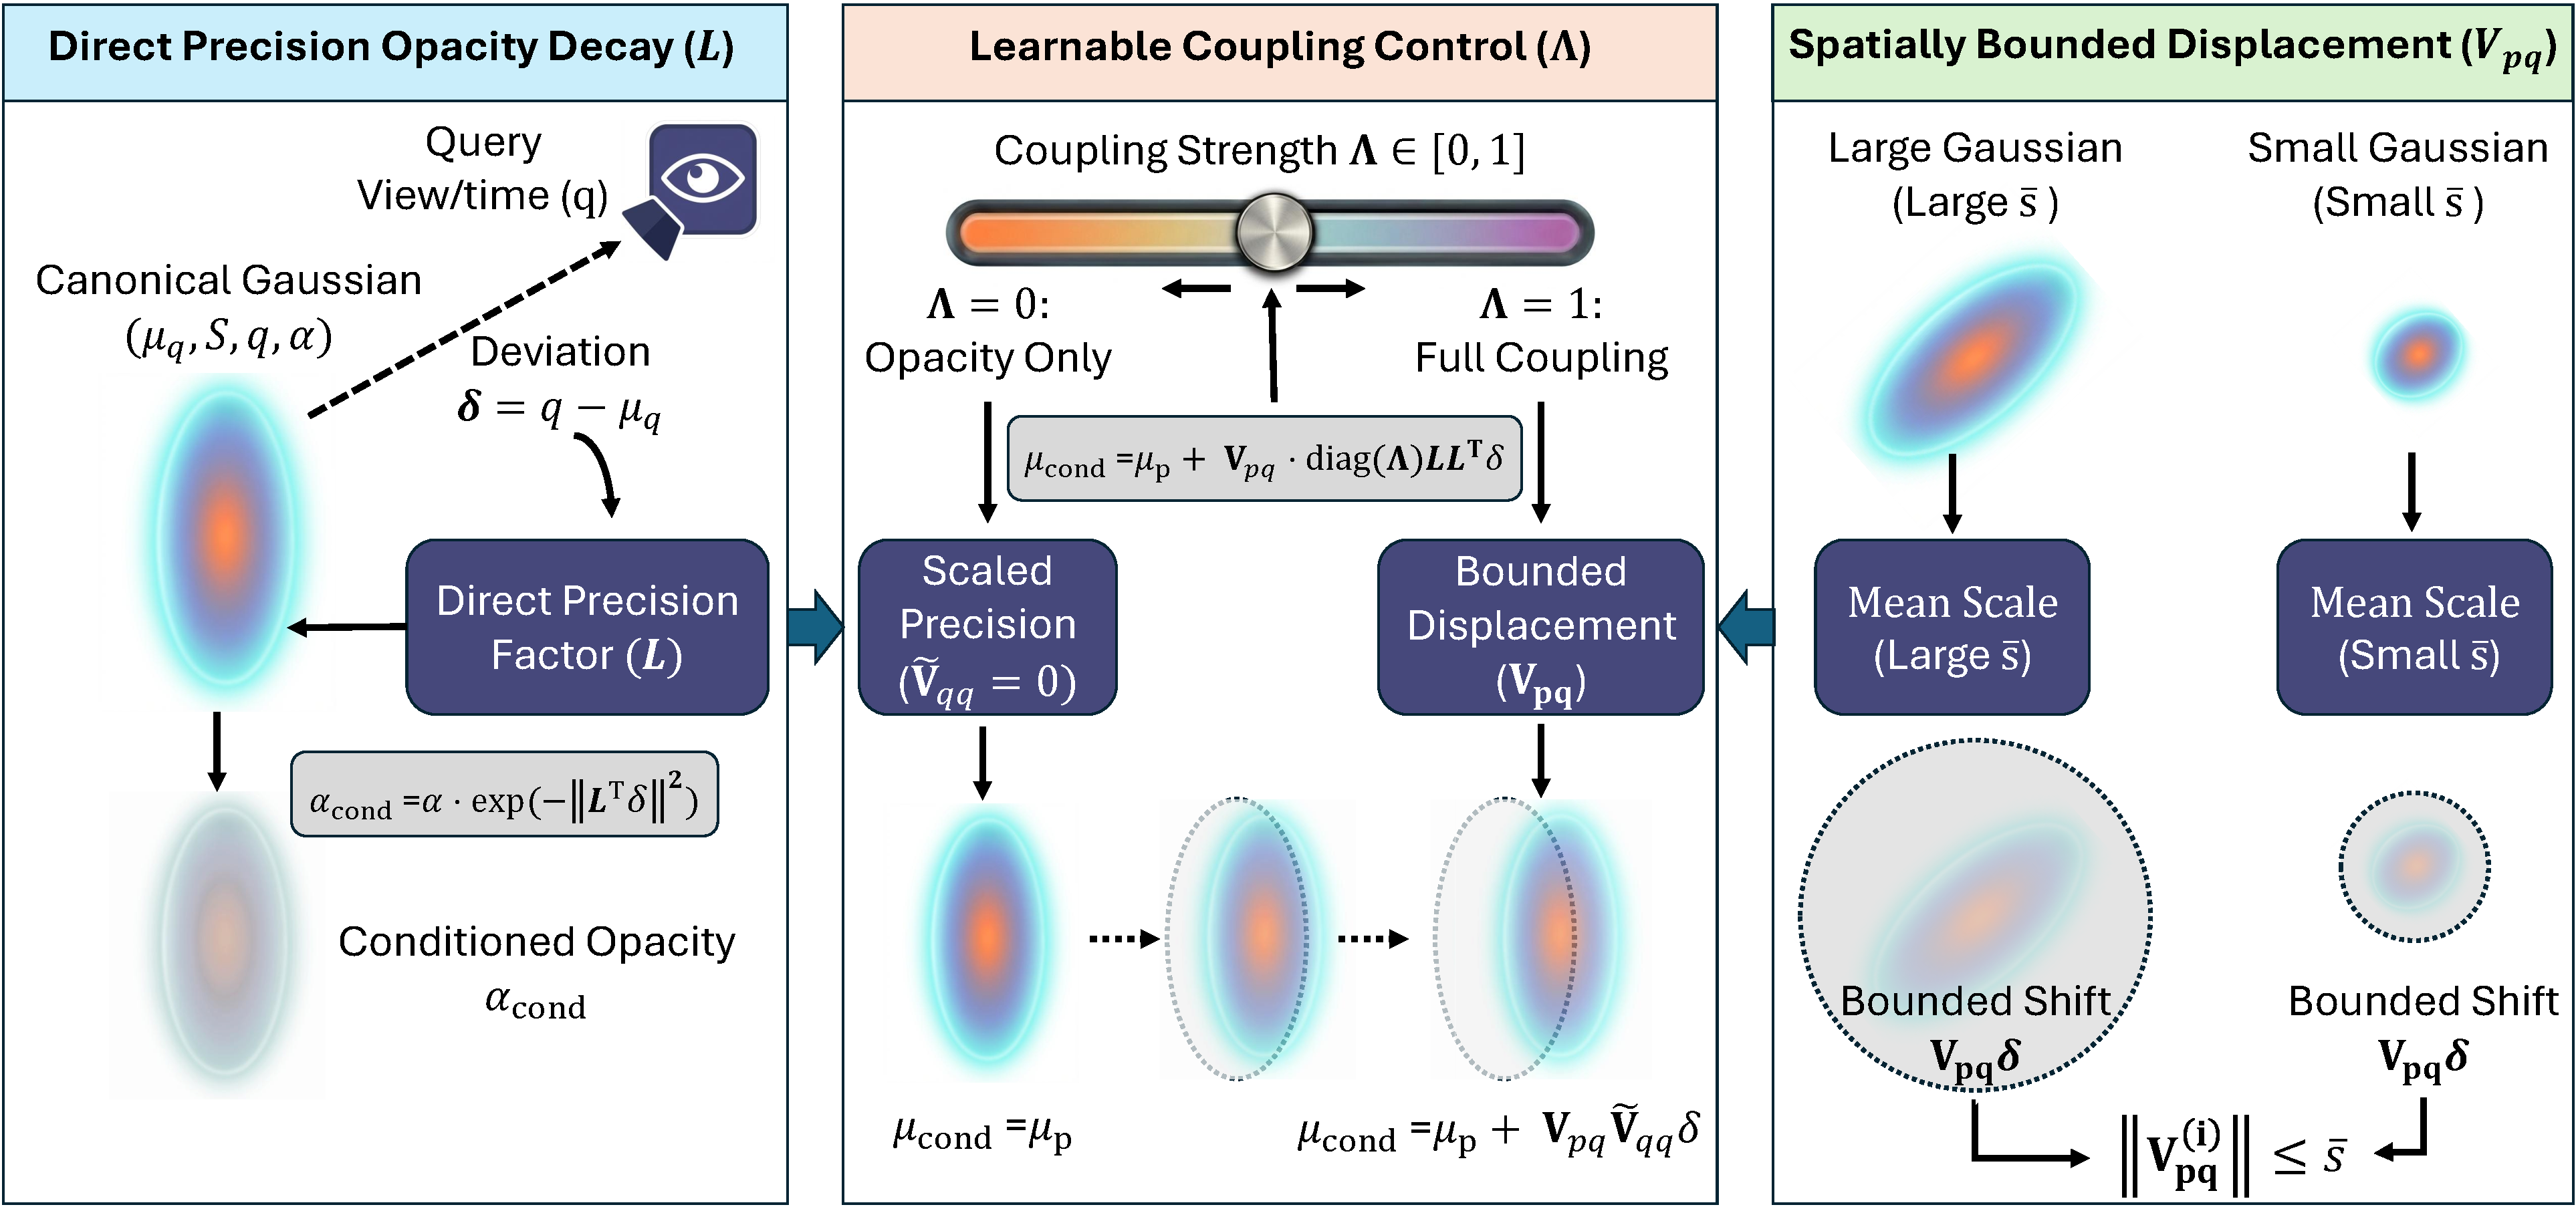
\includegraphics[width=0.99\linewidth]{figures/pipeline.pdf} % Ensure this figure exists
\caption{Overview of the \dgs{} pipeline. Given query deviation $\boldsymbol{\delta} = \mathbf{q} - \boldsymbol{\mu}_q$ from the canonical view/time, we directly parameterize two conditioning effects: (1) \textbf{Opacity modulation} via Cholesky factor $\mathbf{L}$, and (2) \textbf{Position displacement} via displacement matrix $\mathbf{V}_{pq}$ and scaled precision $\tilde{\mathbf{V}}_{qq}$ with learnable per-dimension coupling $\boldsymbol{\Lambda}$. The spatial covariance $\boldsymbol{\Sigma}_{pp}$ remains query-independent. This eliminates matrix inversions and covariance corrections; the same pipeline extends to the Beta kernel as \dbs{} (\cref{subsec:dbs}).}
\label{fig:architecture}
\vspace{-1em}
\end{figure*}

\section{Our Approach}

We replace the covariance-derived conditioning step with three explicit parameters per primitive: a Cholesky factor $\mathbf{L}$ for opacity precision, a displacement matrix $\mathbf{V}_{pq}$ for position, and a per-dimension coupling vector $\boldsymbol{\Lambda}$ that ties the two. We develop the formulation for the Gaussian kernel below, yielding \dgs{}, and show in \cref{subsec:dbs} that swapping in the Beta opacity decay yields \dbs{}.

\subsection{Overview}
\label{subsec:overview}

Given the deviation $\boldsymbol{\delta} = \mathbf{q} - \boldsymbol{\mu}_q$ from the canonical view/time, \dgs{} replaces \cref{eq:prelim_mu,eq:prelim_alpha} with two directly parameterized components:
\begin{align}
\alpha_{\text{cond}} &= \alpha \cdot \exp\!\left(-\lambda_o\,\|\mathbf{L}^\top\boldsymbol{\delta}\|_2^2\right), & &\text{(Opacity)} \label{eq:direct_alpha}\\
\boldsymbol{\mu}_{\text{cond}} &= \boldsymbol{\mu}_p + \mathbf{V}_{pq}\,\mathrm{diag}(\boldsymbol{\Lambda})\,\mathbf{V}_{qq}\,\boldsymbol{\delta}. & &\text{(Position)} \label{eq:direct_mu}
\end{align}
The parameterization is defined by three learned quantities ($\mathbf{L}$, $\mathbf{V}_{pq}$, $\boldsymbol{\Lambda}$) and one fixed constant ($\lambda_o{=}0.35$, the opacity scaling factor inherited from N-DGS). $\mathbf{L}\in\mathbb{R}^{C\times C}$ is a lower-triangular Cholesky factor with an exponential activation on the diagonal, so that $\mathbf{V}_{qq}=\mathbf{L}\mathbf{L}^\top$ is symmetric positive-definite by construction and \emph{is} the precision matrix without any inversion. $\mathbf{V}_{pq}=\bar{s}\boldsymbol{\Theta}_{pq}\in\mathbb{R}^{3\times C}$ is the displacement matrix, written as the average spatial scale $\bar{s}=\mathrm{mean}(s_x,s_y,s_z)$ times a learnable direction $\boldsymbol{\Theta}_{pq}$ with unit Frobenius norm; the spatial-scale prefactor keeps the magnitude of position shifts proportional to the primitive's own size. $\boldsymbol{\Lambda}\in[0,1]^C$ contains per-dimension coupling strengths between opacity and position: at $\boldsymbol{\Lambda}=\mathbf{0}$ position decouples entirely, at $\boldsymbol{\Lambda}=\mathbf{1}$ it couples through the full opacity precision $\mathbf{V}_{qq}$, and intermediate values mix the two per dimension. Dimensions of the same type (\eg, the three view dimensions) share a logit.

The spatial covariance $\boldsymbol{\Sigma}_{pp}=\mathbf{R}\mathbf{S}\mathbf{S}^\top\mathbf{R}^\top$ remains query-independent and unchanged from 3DGS, preserving compatibility with existing densification strategies. For $C=4$ (view and time), $\mathbf{L}$ is constrained to be block-diagonal so that view and time precision do not couple; we expand this in the next subsection. The following two subsections justify the design choices behind $\mathbf{L}$ (opacity) and $\mathbf{V}_{pq}$ with $\boldsymbol{\Lambda}$ (position).


\begin{table}[t!]
\centering
\caption{Per-primitive operations and slicing-only forward pass time on A100 (1M Gaussians) for the four methods spanning implicit/direct conditioning and Gaussian/Beta kernels. Direct methods eliminate inversion, regression, and covariance correction. Speedup factors over the implicit baseline are shown in parentheses.}
\label{tab:comparison_overview}
\setlength{\tabcolsep}{3pt}
\resizebox{0.95\textwidth}{!}{%
\begin{tabular}{@{}l|cc|ccc@{}}
\toprule
& \multicolumn{2}{c|}{\textbf{Implicit}} & \multicolumn{3}{c}{\textbf{Direct (ours)}} \\
\textbf{Operation} & \textbf{N-DGS} & \textbf{UBS} & \textbf{\dgso{}} & \textbf{\dgs{}} & \textbf{\dbs{}} \\
\midrule
Invert $\boldsymbol{\Sigma}_{qq}$ & $\boldsymbol{\Sigma}_{qq}^{-1}$ & $\boldsymbol{\Sigma}_{qq}^{-1}$ & --- & --- & --- \\
Regr.\ matrix $\mathbf{P}$ & $\boldsymbol{\Sigma}_{pq}\boldsymbol{\Sigma}_{qq}^{-1}$ & $\boldsymbol{\Sigma}_{pq}\boldsymbol{\Sigma}_{qq}^{-1}\!\mathrm{diag}(\boldsymbol{\beta}_q)$ & --- & --- & --- \\
Cov.\ correction & $\mathbf{P}\,\boldsymbol{\Sigma}_{pq}^\top$ & $\mathbf{P}\,\boldsymbol{\Sigma}_{pq}^\top$ & --- & --- & --- \\
Position shift & $\mathbf{P}\,\boldsymbol{\delta}$ & $\mathbf{P}\,\boldsymbol{\delta}$ & --- & $\mathbf{V}_{pq}\mathrm{diag}(\boldsymbol{\Lambda})\mathbf{V}_{qq}\boldsymbol{\delta}$ & $\mathbf{V}_{pq}\mathrm{diag}(\boldsymbol{\Lambda}_\beta)\mathbf{V}_{qq}\boldsymbol{\delta}$ \\
Opacity & $\mathcal{K}_G(\boldsymbol{\delta}^\top\!\boldsymbol{\Sigma}_{qq}^{-1}\!\boldsymbol{\delta})$ & $\mathcal{K}_B(\hat{\mathbf{L}}_q^{-1}\!\boldsymbol{\delta};\boldsymbol{\beta})$ & $\mathcal{K}_G(\|\mathbf{L}^\top\!\boldsymbol{\delta}\|^2)$ & $\mathcal{K}_G(\|\mathbf{L}^\top\!\boldsymbol{\delta}\|^2)$ & $\mathcal{K}_B(\mathbf{L}^\top\!\boldsymbol{\delta};\boldsymbol{\beta})$ \\
\midrule
Slicing time, $C{=}3$ (ms) & 0.71 & 0.67 & \textbf{0.08} ($\bm{9.4\times}$) & \textbf{0.10} ($\bm{7.1\times}$) & \textbf{0.10} ($\bm{6.9\times}$) \\
Slicing time, $C{=}4$ (ms) & 0.96 & 1.34 & \,\, \textbf{0.09} ($\bm{10.8\times}$) & \textbf{0.12} ($\bm{7.7\times}$) & \textbf{0.13} ($\bm{7.2\times}$) \\
\bottomrule
\end{tabular}%
}
\vspace{-1em}
\end{table}

Table~\ref{tab:comparison_overview} contrasts the per-primitive operations: N-DGS and UBS pay for the inversion, the regression matrix $\mathbf{P}=\boldsymbol{\Sigma}_{pq}\boldsymbol{\Sigma}_{qq}^{-1}$, and the covariance correction; the direct methods carry none of these. Beyond cost reduction, the per-dimension coupling $\boldsymbol{\Lambda}$ adds a knob that the covariance-derived form does not have: $\boldsymbol{\Lambda}=\mathbf{0}$ recovers an opacity-only variant we denote \dgso{} ($\boldsymbol{\mu}_{\text{cond}}=\boldsymbol{\mu}_p$); $\boldsymbol{\Lambda}=\mathbf{1}$ recovers the same coupling structure as N-DGS but through $\mathbf{V}_{pq}$ rather than $\boldsymbol{\Sigma}_{pq}$; intermediate values give per-dimension partial coupling.

\subsection{Opacity Conditioning}

The Cholesky factor $\mathbf{L}$ is parameterized directly, with exponential activation on the diagonal so that $\mathbf{V}_{qq}=\mathbf{L}\mathbf{L}^\top$ is always symmetric positive-definite. Evaluating opacity reduces to a triangular matrix-vector product $\mathbf{L}^\top\boldsymbol{\delta}$ followed by a squared norm: no inversion, no ill-conditioning of $\boldsymbol{\Sigma}_{qq}$ to worry about.

For $C=4$ (view+time), we constrain $\mathbf{L}$ to be block-diagonal so that view and time precision are independent, reflecting the physical intuition that view-dependent and temporal effects are separate phenomena. With $\boldsymbol{\delta}=(\boldsymbol{\delta}_v,\delta_t)^\top$, opacity factors as
\begin{equation}
\alpha_{\text{cond}} = \alpha \cdot \exp\!\left(-\lambda_o\left(\boldsymbol{\delta}_v^\top \mathbf{V}_{vv} \boldsymbol{\delta}_v + \delta_t^2 v_t\right)\right),
\end{equation}
where $\mathbf{V}_{vv}\in\mathbb{R}^{3\times 3}$ is parameterized by a $3\times 3$ Cholesky factor (6 parameters) and $v_t\in\mathbb{R}$ is a single scalar, for 7 parameters instead of 10 for a full $4\times 4$ precision.

\subsection{Position Conditioning}
\label{subsec:position}

The position update~\eqref{eq:direct_mu} factors into the displacement matrix $\mathbf{V}_{pq}$, the per-dimension coupling $\mathrm{diag}(\boldsymbol{\Lambda})$, and the precision $\mathbf{V}_{qq}$ shared with opacity:
\begin{equation*}
\boldsymbol{\mu}_{\text{cond}} = \boldsymbol{\mu}_p + \underbrace{\bar{s}\,\boldsymbol{\Theta}_{pq}}_{\mathbf{V}_{pq}}\,\underbrace{\mathrm{diag}(\boldsymbol{\Lambda})\,\mathbf{V}_{qq}}_{\tilde{\mathbf{V}}_{qq}}\,\boldsymbol{\delta}.
\end{equation*}
The coupling $\boldsymbol{\Lambda}$ interpolates between two extremes per primitive: at $\boldsymbol{\Lambda}=\mathbf{0}$, position is query-independent (recovering \dgso{}); at $\boldsymbol{\Lambda}=\mathbf{1}$, position and opacity share the full precision $\mathbf{V}_{qq}$, mirroring N-DGS's coupling structure. Different query dimensions (view vs.\ time) can choose different coupling strengths during training.

\textbf{Spatial scaling.} Following N-DGS's principle that displacement should scale with spatial extent, we set $\mathbf{V}_{pq}=\bar{s}\,\boldsymbol{\Theta}_{pq}$ with $\|\boldsymbol{\Theta}_{pq}\|_F=1$, so that the displacement of each spatial row is uniformly bounded by the primitive's own average size: $\|\mathbf{V}_{pq}^{(i)}\|_2\le\bar{s}$. The covariance-derived displacement in N-DGS is bounded by $\sqrt{C}(i-1+s_i)$ instead, which contains an additive constant $(i-1)\sqrt{C}$ that does not shrink with $s_i$: small Gaussians can still produce displacements far larger than their own extent. The bound is also asymmetric across spatial rows (it grows with the row index $i$), which makes the magnitude of position shifts depend on dimension ordering. Our explicit form removes both effects in one step. Appendix~\ref{sec:spatial_scaling_proof} gives the derivation; the ablation in \cref{tab:ablation} confirms the design empirically: removing $\bar{s}$ degrades PSNR by 2.65 dB on NeRF Synthetic.




\subsection{Extension to Beta Kernel: \dbs{}}
\label{subsec:dbs}

Direct conditioning touches only the slicing step (precision read-out, displacement, and coupling), making it kernel-agnostic: any opacity decay that consumes the precision-Cholesky distance $\mathbf{L}^\top\boldsymbol{\delta}$ can be substituted in. We instantiate this with UBS's Beta kernel~\citep{liu2025universal} to obtain \dbs{} (direct Beta Splatting), the direct counterpart of UBS.

UBS evaluates opacity as $\alpha\cdot\prod_i (1-\tanh((\hat{\mathbf{L}}_q^{-1}\boldsymbol{\delta})_i^2/2))^{4\beta_i}$, where $\hat{\mathbf{L}}_q$ is the Cholesky factor of $\boldsymbol{\Sigma}_{qq}$ obtained by inverting/back-substituting against the covariance, and $\boldsymbol{\beta}\in\mathbb{R}^C$ is the per-dimension Beta bandwidth. \dbs{} replaces the back-substitution $\hat{\mathbf{L}}_q^{-1}\boldsymbol{\delta}$ with our direct Cholesky product $\mathbf{z}=\mathbf{L}^\top\boldsymbol{\delta}$:
\begin{align}
\alpha_{\text{cond}} &= \alpha \cdot \prod_{i=1}^{C} \bigl(1-\tanh(z_i^2)\bigr)^{\beta_i}, \label{eq:dbs_alpha}\\
\boldsymbol{\mu}_{\text{cond}} &= \boldsymbol{\mu}_p + \mathbf{V}_{pq}\,\mathrm{diag}(\boldsymbol{\Lambda}_\beta)\,\mathbf{V}_{qq}\,\boldsymbol{\delta}, \label{eq:dbs_mu}
\end{align}
where $\beta_i = 4\exp(\beta_i^{\text{raw}})$ for unconstrained learnable parameters $\beta_i^{\text{raw}}\in\mathbb{R}$ (the $4\exp(\cdot)$ activation matches UBS, ensuring $\beta_i > 0$ and giving a smooth gradient for bandwidth control). The position update~\eqref{eq:dbs_mu} mirrors \cref{eq:direct_mu}, but reuses the \emph{same} $\boldsymbol{\beta}$ that drives opacity bandwidth as the source of position coupling. We rescale it to $\boldsymbol{\Lambda}_\beta = \min(\boldsymbol{\beta}/4,\,\mathbf{1})$ so that the coupling lies in $[0,1]$ and plays the same role as \dgs{}'s learned $\boldsymbol{\Lambda}$. Sharing $\boldsymbol{\beta}$ between opacity bandwidth and position coupling saves one parameter set per primitive relative to \dgs{}. All other components ($\mathbf{L}$, $\mathbf{V}_{pq}$, $\boldsymbol{\Sigma}_{pp}$, and the block-diagonal view/time structure) transfer unchanged from \dgs{}. Appendix~\ref{sec:dbs} gives the full side-by-side derivation against UBS.

\subsection{CUDA Implementation}

The original N-DGS methods (6DGS~\cite{gao20246dgs}, 7DGS~\cite{gao20257dgs}) rely on PyTorch's autograd for the conditional Gaussian operations, so for a fair comparison we implement \dgs{} and the N-DGS baseline with custom CUDA kernels. The kernel fuses the conditional position and opacity computation in a single pass (Algorithm~\ref{alg:slice} in Appendix~\ref{sec:algorithms}), and \dbs{} reuses the same pipeline with the opacity decay swapped (Algorithm~\ref{alg:slice_dbs}).

\textbf{Kernel design.} The kernel is templated on $C$ ($3$ or $4$) with compile-time loop unrolling, and each thread processes one primitive. The triangular product $\mathbf{L}^\top\boldsymbol{\delta}$ uses only $C(C+1)/2$ multiplications followed by a dot product, all in per-thread registers; the small $3\times C$ and $C\times C$ matrices fit entirely in registers, so the kernel allocates no intermediate tensors and avoids shared-memory traffic.

\begin{figure*}[!t]
    \centering
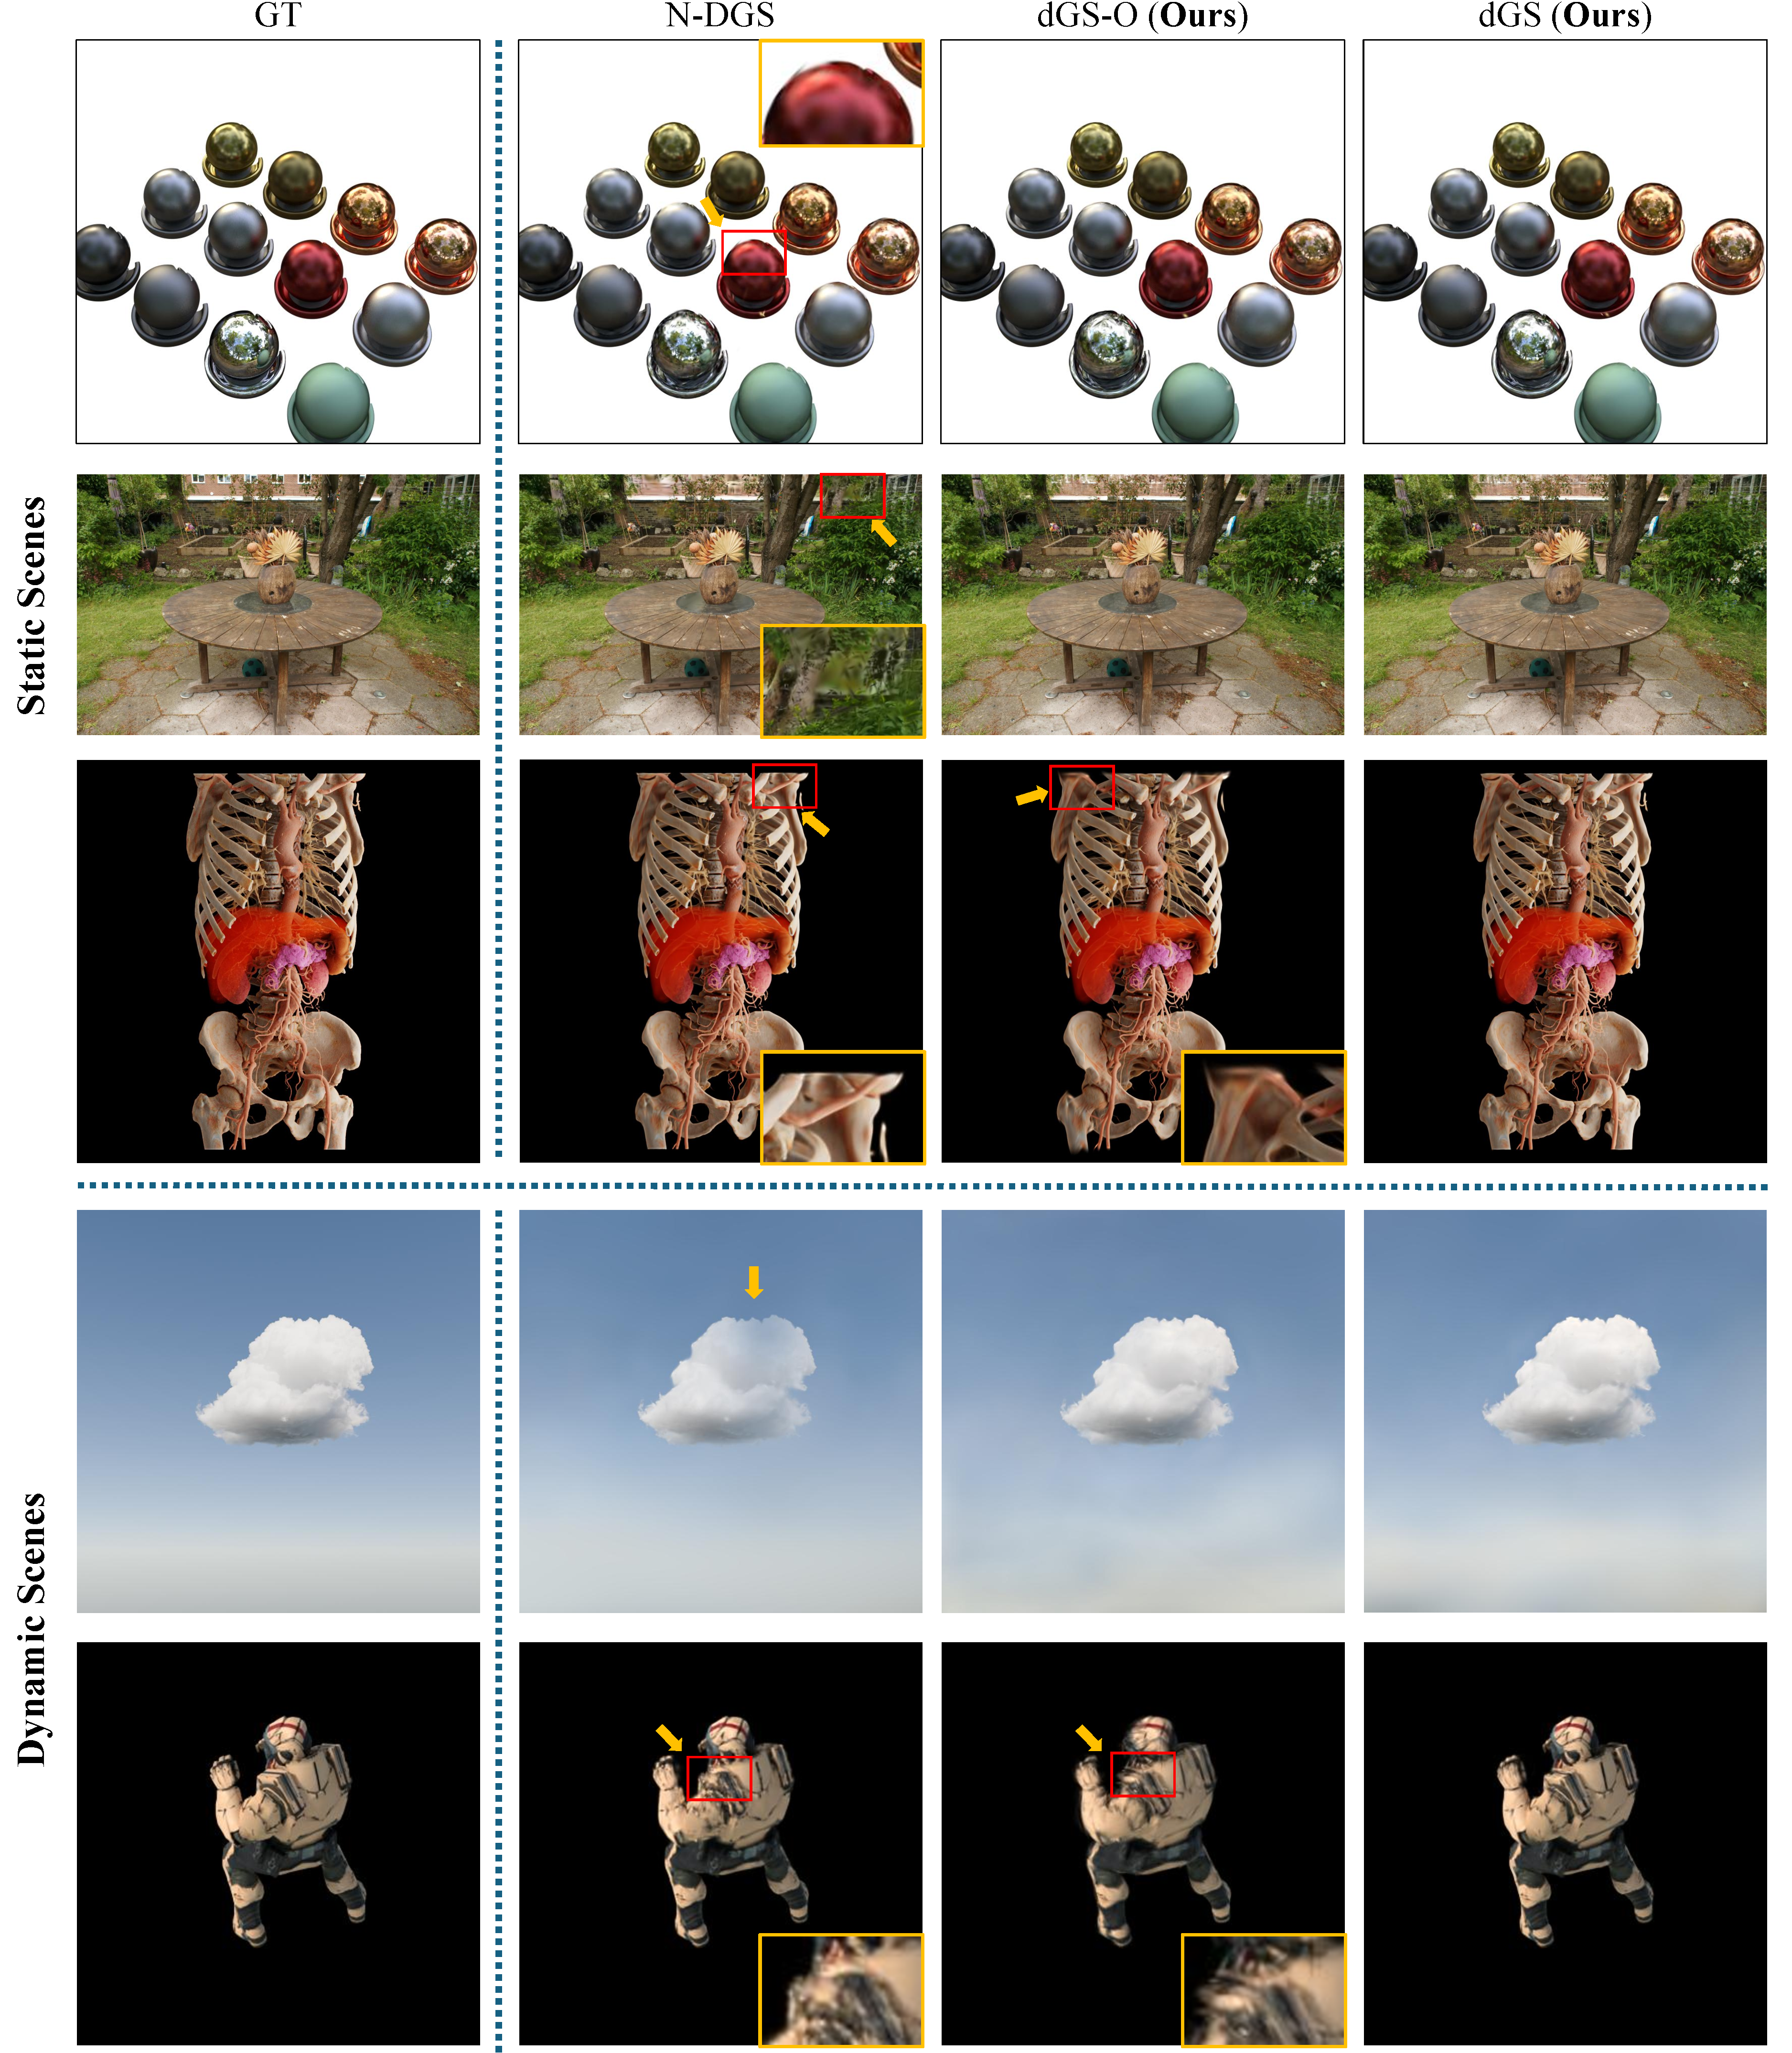
\includegraphics[width=0.85\linewidth]{figures/qualitative.pdf}
    \caption{Qualitative comparison of methods for static and dynamic scenes (zoom in for details).}
    \label{fig:qualitative}
    \vspace{-1em}
\end{figure*}

\textbf{Kernel benchmarks.} The slicing-time rows of Table~\ref{tab:comparison_overview} report the raw CUDA forward pass (no autograd overhead) at 1M Gaussians on an A100, isolating slicing from rasterization and densification. Direct conditioning is consistently \textbf{7--8$\times$ faster} (\dgs{}, \dbs{}) and \textbf{9--11$\times$ faster} (\dgso{}) than the covariance-derived baselines across $C{=}3$ and $C{=}4$. End-to-end rendering achieves up to 2.66$\times$ speedup (Appendix~\ref{sec:detailed_results}, Table~\ref{tab:summary_results}); the remaining time is dominated by rasterization, which is shared across all methods.


\begin{table*}[t]
\centering
\caption{MCMC densification on static and dynamic datasets; means across all scenes (\#Gauss in K, time in minutes). FPS and FPS$_{\text{CUDA}}$ both use the TC-GS~\citep{liao2025tc} rasterizer but differ in the slicing implementation: FPS uses a PyTorch reference, FPS$_{\text{CUDA}}$ uses our fused CUDA kernels. We follow the 3DGS~\citep{3dgs} evaluation protocol (joint-RGB test PSNR, white background on NeRF Synthetic); UBS numbers therefore differ from~\citep{liu2025universal}, which uses channel-averaged PSNR and a black background for NeRF Synthetic.}
\label{tab:mcmc_comparison}
\resizebox{0.85\textwidth}{!}{%
\begin{tabular}{@{}ccl|rrrr|ccc@{}}
\toprule
& Dataset & Method & \#Gauss & Time $\downarrow$ & FPS $\uparrow$& FPS$_{\text{CUDA}}$ $\uparrow$& PSNR $\uparrow$ & SSIM $\uparrow$ & LPIPS $\downarrow$ \\
\midrule
\multirow{12}{*}{\rotatebox{90}{STATIC}}
& \multirow{4}{*}{\makecell{\texttt{NeRF}\\\texttt{Synthetic}}}
& N-DGS & 300 & 10.43 & 183.58 & 348.95 & 34.04 & 0.973 & 0.027 \\
&& \textit{d}GS (\textbf{Ours}) & 300 & \bf 10.26 & \bf 245.18 & \bf 593.94 &  \bf 34.34 &  \bf 0.973 &  \bf 0.026 \\
\spacedcdashline{3-10}
&& UBS & 300 & 6.80 & 155.96 & 306.33 & 34.48 & 0.975 & 0.026 \\
&& \textit{d}BS (\textbf{Ours}) & 300 &  \bf5.48 & \bf 239.09 &  \bf 415.66 & \bf 34.53 & \bf 0.975 & \bf 0.025 \\
\cmidrule{2-10}
& \multirow{4}{*}{\makecell{\texttt{Mip-NeRF}\\\texttt{360}}}
& N-DGS & 2,852 & 51.23 & 35.69 & 75.31 & 26.88 & 0.775 & 0.263 \\
&& \textit{d}GS (\textbf{Ours}) & 2,574 & \bf 49.85 & \bf 42.49 & \bf 200.56 &  \bf 27.67 & \bf 0.794 & \bf  0.227 \\
\spacedcdashline{3-10}
&& UBS & 3,057 & 28.59 & 40.94 & 76.18 & 28.50 & 0.841 & \bf 0.183 \\
&& \textit{d}BS (\textbf{Ours}) & 3,057 &  \bf 24.42 & \bf 62.05 &  \bf 157.45 & \bf 28.70 & \bf 0.842 & 0.185 \\
\cmidrule{2-10}
& \multirow{4}{*}{\texttt{6DGS-PBR}}
& N-DGS & 163 & 54.80 & 328.75 & 476.79 & 40.06 & 0.976 & 0.039 \\
&& \textit{d}GS (\textbf{Ours}) & 163 & \bf 47.54 & \bf 356.15 & \bf 551.02 & \bf 40.34 & \bf 0.976 & \bf 0.038 \\
\spacedcdashline{3-10}
&& UBS & 163 & 8.70 & 239.87 & 348.63 & 39.53 & 0.975 & 0.042 \\
&& \textit{d}BS (\textbf{Ours}) & 163 & \bf 8.47 & \bf 305.33 & \bf 401.93 & \bf 39.72 & \bf 0.976 & \bf 0.042 \\
\midrule
\midrule
\multirow{8}{*}{\rotatebox{90}{DYNAMIC}}
& \multirow{4}{*}{\texttt{D-NeRF}}
& N-DGS & 150 & \bf 10.31 & 306.51 & 501.52 & 34.63 & 0.976 & 0.033 \\
&& \textit{d}GS (\textbf{Ours}) & 150 &  10.61 & \bf 407.40 & \bf 746.65 & \bf 34.64 & \bf 0.976 & \bf 0.030 \\
\spacedcdashline{3-10}
&& UBS & 150 & \bf 8.37 & 229.83 & 371.81 & 32.91 & 0.967 & 0.040 \\
&& \textit{d}BS (\textbf{Ours}) & 150 & 9.34 & \bf 323.75 & \bf 463.09 & \bf 33.55 & \bf 0.972 & \bf 0.033 \\
\cmidrule{2-10}
& \multirow{4}{*}{\texttt{7DGS-PBR}}
& N-DGS & 175 & \bf 28.44 & 294.48 & 511.12 & 29.20 & 0.944 & 0.063 \\
&& \textit{d}GS (\textbf{Ours}) & 175 & 31.12 & \bf 366.06 & \bf 577.38 & \bf 29.90 & \bf 0.948 & \bf 0.061 \\
\spacedcdashline{3-10}
&& UBS & 175 & 9.90 & 232.17 & 396.33 & 30.61 & 0.951 & 0.057 \\
&& \textit{d}BS (\textbf{Ours}) & 175 & \bf 8.79 & \bf 347.93 & \bf 539.57 & \bf 31.87 & \bf 0.955 & \bf 0.053 \\
\bottomrule
\end{tabular}}
\end{table*}




\section{Experiments}
\label{sec:experiments}

\subsection{Experimental Setup}

\textbf{Datasets.}
We evaluate the \dfamily{} family across five diverse datasets covering both static and dynamic scenes:
\vspace{-1em}
\begin{itemize}[leftmargin=*]
    \item \textit{Static scenes:} (1) \textit{NeRF Synthetic}~\cite{mildenhall2021nerf} with 8 synthetic scenes under controlled lighting for evaluating geometric reconstruction; (2) \textit{Mip-NeRF 360}~\cite{barron2021mipnerf} with 9 challenging unbounded real-world scenes for evaluating view synthesis; and (3) \textit{6DGS-PBR}~\cite{gao20246dgs} featuring 7 physically-based scenes with complex view-dependent effects.

    \item \textit{Dynamic scenes:} (4) \textit{D-NeRF}~\cite{pumarola2020dnerfneuralradiancefields} with 8 synthetic sequences featuring various deformation types; and (5) \textit{7DGS-PBR}~\cite{gao20257dgs} containing 6 physically-based dynamic scenes with complex spatio-temporal-angular correlations.
\end{itemize}


\textbf{Evaluation Metrics.}
We assess reconstruction quality using Peak Signal-to-Noise Ratio (PSNR), Structural Similarity Index (SSIM)~\cite{wang2004image}, and Learned Perceptual Image Patch Similarity (LPIPS)~\cite{zhang2018perceptual}. We also report rendering speed (FPS), training time (minutes), and Gaussian count (K) to evaluate computational efficiency.

\textbf{Implementation Details.}
All methods are implemented in PyTorch with custom CUDA kernels on a single NVIDIA A100 GPU and rendered with the TC-GS rasterizer~\citep{liao2025tc}. We compare two head-to-head pairs (\dgs{} vs.\ N-DGS, \dbs{} vs.\ UBS) and additionally include \dgso{} (\dgs{} with $\boldsymbol{\Lambda}{=}\mathbf{0}$) as a maximum-efficiency variant. All methods share the same training pipeline: Adam optimizer, 30K iterations, identical learning rates and densification schedules per dataset. For \dgs{} and \dbs{}, the view mean $\boldsymbol{\mu}_q$ is initialized to random unit vectors (with time uniformly sampled in $[0,1]$ for dynamic scenes), the displacement parameters $\boldsymbol{\Theta}_{pq}$ from $\mathcal{N}(0,0.01^2)$, and the Cholesky factor $\mathbf{L}$ with diagonal elements $\log(2.0)$ and zero off-diagonals.

\subsection{Results with MCMC Densification}

Table~\ref{tab:mcmc_comparison} compares each direct method against its covariance-derived counterpart under MCMC densification~\citep{kheradmand20243dgaussiansplattingmarkov}. Each row pair uses an identical Gaussian budget so any difference reflects the conditioning parameterization rather than primitive count. Following the original settings, we cap primitives at 300K for NeRF Synthetic and 150K for D-NeRF, and use scene-specific caps depending on scene complexity for Mip-NeRF 360 (1.5M--6M), 6DGS-PBR (60K--300K), and 7DGS-PBR (150K--300K).

\textbf{Gaussian-kernel pair (\dgs{} vs.\ N-DGS).} Direct conditioning improves quality on every dataset and delivers large rendering speedups, with the gap widening as the scene grows. On the largest benchmark, Mip-NeRF 360, \dgs{} achieves +0.79 dB PSNR and +166\% FPS$_{\text{CUDA}}$ (200.56 vs.\ 75.31). On NeRF Synthetic, +0.30 dB and +70\% (593.94 vs.\ 348.95). On the dynamic side, D-NeRF gives near-identical quality (+0.01 dB) but +49\% rendering speed (746.65 vs.\ 501.52); 7DGS-PBR adds dynamics on top of view-dependent specular effects, where \dgs{} both improves quality (+0.70 dB) and renders +13\% faster (577.38 vs.\ 511.12).

\textbf{Beta-kernel pair (\dbs{} vs.\ UBS).} The same advantage transfers to the Beta kernel. On NeRF Synthetic, \dbs{} matches UBS quality (+0.05 dB) while rendering +36\% faster (415.66 vs.\ 306.33) and training in 5.48 vs.\ 6.80 minutes. On Mip-NeRF 360, \dbs{} improves PSNR by +0.20 dB and renders +107\% faster (157.45 vs.\ 76.18). On D-NeRF, \dbs{} delivers a substantial +0.64 dB gain with +25\% faster rendering (463.09 vs.\ 371.81). The 7DGS-PBR gap is largest: +1.26 dB and +36\% (539.57 vs.\ 396.33), with per-scene PSNR gains reaching +2.06 dB on \texttt{heart}. Across all four datasets the speedup pattern matches the Gaussian-kernel pair, confirming the gains come from removing covariance-derived conditioning rather than from kernel-specific tricks.

\textbf{Slicing kernel matters most for large scenes.} The two FPS columns isolate the contribution of our CUDA slicing kernel from rasterization: both use the same TC-GS rasterizer, but FPS uses a PyTorch reference for slicing while FPS$_{\text{CUDA}}$ uses our fused kernel. On small scenes, slicing is only a small fraction of the per-frame cost, so the CUDA speedup is modest (1.90$\times$ for N-DGS on NeRF Synthetic). On Mip-NeRF 360, where the kernel runs on millions of primitives per frame, the slicing kernel dominates: $2.11\times$ for N-DGS, and $4.72\times$ for \dgs{} (200.56 vs.\ 42.49). The same trend holds for the Beta-kernel pair (\eg, \dbs{} at 463.09 vs.\ 323.75 on D-NeRF, $1.43\times$).

Figure~\ref{fig:qualitative} shows qualitative comparisons: \dgs{} and \dbs{} reconstruct fewer artifacts than their covariance-derived baselines on both static and dynamic scenes. Standard-densification results for \dgs{} vs.\ N-DGS, the protocol N-DGS originally evaluates with, appear in Appendix~\ref{sec:detailed_results}.

\begin{table}[!t]
\centering
\caption{Ablation study on NeRF Synthetic and 6DGS-PBR datasets. $\Lambda{=}0$ corresponds to \textit{d}GS-O (opacity only), $\Lambda{=}1$ fixes full coupling, and learned $\Lambda$ is the full \textit{d}GS. ``w/o $\bar{s}$'' removes spatial scaling from displacement.}
\label{tab:ablation}
\setlength{\tabcolsep}{4pt}
\resizebox{0.7\textwidth}{!}{%
\begin{tabular}{l|ccc|ccc}
\toprule
 & \multicolumn{3}{c|}{\texttt{NeRF Synthetic}} & \multicolumn{3}{c}{\texttt{6DGS-PBR}} \\
Config & PSNR $\uparrow$ & SSIM $\uparrow$ & LPIPS $\downarrow$ & PSNR $\uparrow$ & SSIM $\uparrow$ & LPIPS $\downarrow$ \\
\midrule
$\Lambda{=}0$ (\textit{d}GS-O) & 33.84 & 0.971 & 0.030 & 36.54 & 0.965 & 0.059 \\
$\Lambda{=}1$ (fixed) & 33.78 & 0.971 & 0.029 & 37.31 & \textbf{0.972} & 0.053 \\
\textit{d}GS w/o $\bar{s}$ & 31.26 & 0.957 & 0.046 & 34.78 & 0.951 & 0.075 \\
$\Lambda$ learned (\textit{d}GS) & \textbf{33.91} & \textbf{0.972} & \textbf{0.029} & \textbf{37.75} & \textbf{0.972} & \textbf{0.052} \\
\bottomrule
\end{tabular}}%
\vspace{-1em}
\end{table}

\subsection{Ablation Study}

Table~\ref{tab:ablation} ablates the two key design choices: the per-dimension coupling $\boldsymbol{\Lambda}$ and the spatial scaling $\bar{s}$ in the displacement matrix. All ablation runs use standard 3DGS densification~\citep{3dgs} on NeRF Synthetic and 6DGS-PBR (the same protocol as the appendix Standard-Densification results).

\textbf{Learned $\boldsymbol{\Lambda}$ outperforms both fixed extremes.} On NeRF Synthetic, learned $\boldsymbol{\Lambda}$ achieves 33.91 dB vs.\ 33.84 ($\boldsymbol{\Lambda}{=}\mathbf{0}$, opacity-only) and 33.78 ($\boldsymbol{\Lambda}{=}\mathbf{1}$, full coupling). The gap widens on 6DGS-PBR (view-dependent specular scenes): 37.75 dB vs.\ 36.54 ($\boldsymbol{\Lambda}{=}\mathbf{0}$, $-1.21$ dB) and 37.31 ($\boldsymbol{\Lambda}{=}\mathbf{1}$, $-0.44$ dB). The optimal coupling is scene-dependent and even primitive-dependent: the diffuse NeRF Synthetic scenes prefer weak coupling ($\boldsymbol{\Lambda}{=}\mathbf{0}$ beats $\boldsymbol{\Lambda}{=}\mathbf{1}$), the specular 6DGS-PBR scenes prefer strong coupling ($\boldsymbol{\Lambda}{=}\mathbf{1}$ beats $\boldsymbol{\Lambda}{=}\mathbf{0}$ by +0.77 dB), and learned per-Gaussian $\boldsymbol{\Lambda}$ improves on both extremes on both datasets.

\textbf{Spatial scaling is critical.} Removing $\bar{s}$ degrades PSNR by 2.65 dB on NeRF Synthetic (33.91 vs.\ 31.26) and 2.97 dB on 6DGS-PBR (37.75 vs.\ 34.78). Notably, displacement \emph{without} spatial scaling is worse than no displacement at all (the $\boldsymbol{\Lambda}{=}\mathbf{0}$ baseline at 33.84 / 36.54 beats \dgs{} w/o $\bar{s}$ at 31.26 / 34.78), showing that unscaled position shifts hurt the model rather than just being neutral. This matches the bound analysis in Appendix~\ref{sec:spatial_scaling_proof}: tying displacement magnitude to the primitive's own spatial extent is what keeps the shift consistent across small and large Gaussians.

\section{Future Work}

Direct conditional parameterization extends naturally to other primitive attributes and other query variables, with the attributes (opacity, position) playing a role analogous to values modulated by queries (view direction, time). Opacity and position are the attributes that current N-dimensional splatting methods condition; rotation and color are the obvious next targets. View direction and time are the current queries; lighting direction and material properties would be natural additions. The framework also extends to other recently proposed kernels such as Student-t~\citep{zhu20253dstudentsplattingscooping}, Gabor~\citep{zhou20253dgabsplat3dgaborsplatting}, and generalized exponentials~\citep{hamdi2024gesgeneralizedexponentialsplatting}, since direct conditioning only requires a kernel that consumes the precision-Cholesky distance $\mathbf{L}^\top\boldsymbol{\delta}$. Each new conditioning effect plugs into the same framework with a directly parameterized projection from the query and a learnable coupling strength, without introducing the matrix inversions and covariance corrections that grow with the joint covariance. The per-primitive cost scales linearly with the number of conditioning effects rather than quadratically with the conditioning dimension.

\section{Conclusion}

We presented direct conditional parameterization for N-dimensional splatting: a kernel-agnostic alternative to the covariance-derived conditioning shared by N-DGS and UBS, which parameterizes opacity precision and position displacement explicitly rather than reading them out of a joint covariance. The conditioning step and the kernel can be improved independently, even though the prior literature treats them as a single design block: improving the conditioning step does not require changing the kernel, and the same improvement carries across kernel families. Replacing the covariance-derived machinery (inversion, regression, correction) with explicit parameters does not cost quality. Instantiated as \dgs{} (Gaussian) and \dbs{} (Beta), the framework matches or exceeds N-DGS and UBS on PSNR across all five static and dynamic benchmarks, runs 6.9--10.8$\times$ faster at the slicing step, and up to 2.66$\times$ faster end-to-end. Direct parameterization is a drop-in replacement for the conditioning step, and its kernel-agnostic, explicit form makes it a natural building block for extending splatting to new kernels, new query variables, and new conditioned attributes.

\makeatletter
\if@neuripsfinal
\begin{ack}
% Fill this section for the final camera-ready version.
\end{ack}
\fi
\makeatother

% References section
\bibliographystyle{plainnat}
\bibliography{references}

%%%%%%%%%%%%%%%%%%%%%%%%%%%%%%%%%%%%%%%%%%%%%%%%%%%%%%%%%%%%%%%%%%%%%%%%%%%%%%%
%%%%%%%%%%%%%%%%%%%%%%%%%%%%%%%%%%%%%%%%%%%%%%%%%%%%%%%%%%%%%%%%%%%%%%%%%%%%%%%
% APPENDIX
%%%%%%%%%%%%%%%%%%%%%%%%%%%%%%%%%%%%%%%%%%%%%%%%%%%%%%%%%%%%%%%%%%%%%%%%%%%%%%%
%%%%%%%%%%%%%%%%%%%%%%%%%%%%%%%%%%%%%%%%%%%%%%%%%%%%%%%%%%%%%%%%%%%%%%%%%%%%%%%
\newpage
\appendix
\section{Conditional Slicing Algorithms}
\label{sec:algorithms}

The fused CUDA kernels for \dgs{} and \dbs{} are summarized below. Both share the same precision-Cholesky distance computation $\mathbf{L}^\top\boldsymbol{\delta}$ and the same direct displacement structure for position; they differ only in the opacity decay function applied to that distance.

\begin{algorithm}[h]
\caption{\dgs{} Conditional Slicing}
\label{alg:slice}
\begin{algorithmic}[1]
\REQUIRE Primitive parameters: $\mu_p$, $\mu_q$, $\alpha$, $\mathbf{S}$, $\boldsymbol{\Theta}_{pq}$, $\mathbf{L}$, $\boldsymbol{\Lambda}$
\REQUIRE Query point: $q$ (view/time)
\STATE $\boldsymbol{\delta} \gets q - \mu_q$
\STATE $\alpha_{\text{cond}} \gets \alpha \cdot \exp(-\lambda_o\,\|\mathbf{L}^\top \boldsymbol{\delta}\|^2)$ \Comment{Gaussian opacity decay}
\IF{\dgso{} variant}
    \STATE \return  $\alpha_{\text{cond}}, \mu_p$ \Comment{Early exit for opacity only}
\ENDIF
\STATE $\mathbf{V}_{pq} \gets \text{mean}(\text{diag}(\mathbf{S})) \cdot \boldsymbol{\Theta}_{pq}$
\STATE $\tilde{\mathbf{V}}_{qq} \gets \mathrm{diag}(\boldsymbol{\Lambda})\,\mathbf{L}\mathbf{L}^\top$
\STATE $\mu_{\text{cond}} \gets \mu_p + \mathbf{V}_{pq} \cdot \tilde{\mathbf{V}}_{qq} \cdot \boldsymbol{\delta}$
\STATE \return $\alpha_{\text{cond}}$, $\mu_{\text{cond}}$
\end{algorithmic}
\end{algorithm}

\begin{algorithm}[h]
\caption{\dbs{} Conditional Slicing}
\label{alg:slice_dbs}
\begin{algorithmic}[1]
\REQUIRE Primitive parameters: $\mu_p$, $\mu_q$, $\alpha$, $\mathbf{S}$, $\boldsymbol{\Theta}_{pq}$, $\mathbf{L}$, $\boldsymbol{\beta}$
\REQUIRE Query point: $q$ (view/time)
\STATE $\boldsymbol{\delta} \gets q - \mu_q$
\STATE $\mathbf{z} \gets \mathbf{L}^\top \boldsymbol{\delta}$
\STATE $\alpha_{\text{cond}} \gets \alpha \cdot \prod_{i=1}^{C} (1 - \tanh(z_i^2))^{\beta_i}$ \Comment{Beta opacity decay}
\STATE $\boldsymbol{\Lambda}_\beta \gets \min(\boldsymbol{\beta}/4,\, \mathbf{1})$ \Comment{Beta-derived coupling}
\STATE $\mathbf{V}_{pq} \gets \text{mean}(\text{diag}(\mathbf{S})) \cdot \boldsymbol{\Theta}_{pq}$
\STATE $\tilde{\mathbf{V}}_{qq} \gets \mathrm{diag}(\boldsymbol{\Lambda}_\beta)\,\mathbf{L}\mathbf{L}^\top$
\STATE $\mu_{\text{cond}} \gets \mu_p + \mathbf{V}_{pq} \cdot \tilde{\mathbf{V}}_{qq} \cdot \boldsymbol{\delta}$
\STATE \return $\alpha_{\text{cond}}$, $\mu_{\text{cond}}$
\end{algorithmic}
\end{algorithm}

\section{Comparison with State-of-the-art Methods}
\label{app:sota}

The main paper compares each direct method against its covariance-derived counterpart in matched pairs to isolate the contribution of conditioning. Here we situate \dbs{} against a broader range of static-scene methods on Mip-NeRF 360~\citep{barron2021mipnerf} and NeRF Synthetic~\citep{mildenhall2021nerf}, including implicit (Instant-NGP, Mip-NeRF 360, Zip-NeRF) and explicit (3DGS family, DBS, UBS) baselines. Table~\ref{tab:sota} reports results: \dbs{}-6D achieves the best PSNR on Mip-NeRF 360 (28.70 dB) and the best LPIPS on NeRF Synthetic (0.025), and is competitive on the remaining metrics. Compared to its covariance-derived counterpart UBS-6D~\citep{liu2025universal}, \dbs{}-6D matches SSIM, slightly improves PSNR and LPIPS on Mip-NeRF 360, and trails on NeRF Synthetic PSNR while improving LPIPS. The point of this comparison is not a single-metric win but to show that direct conditioning, despite removing the entire covariance-derived machinery, remains competitive with the strongest published baselines on both benchmarks.

\begin{table*}[thp]
    \centering
    \caption{Comparison with SOTA methods on Mip-NeRF360~\citep{barron2021mipnerf} and NeRF Synthetic~\citep{mildenhall2021nerf}. UBS and \textit{d}BS are evaluated under the 3DGS protocol.}
    \resizebox{0.95\linewidth}{!}{%
    \begin{tabular}{cl|ccc|ccc}
        \toprule
        & \multirow{2}{*}{Methods}
        & \multicolumn{3}{c|}{Mip-NeRF360}
        & \multicolumn{3}{c}{NeRF Synthetic}\\
        \cmidrule(lr){3-8}
         &
         & PSNR$\uparrow$ & SSIM$\uparrow$ & LPIPS$\downarrow$
         & PSNR$\uparrow$ & SSIM$\uparrow$ & LPIPS$\downarrow$ \\
        \midrule
        \parbox[t]{2mm}{\multirow{3}{*}{\rotatebox[origin=c]{90}{implicit}}}
         & Instant-NGP~\citep{M_ller_2022}
           & 25.51 & 0.684 & 0.398
           &33.18 & 0.959&0.055\\
         & Mip-NeRF360~\citep{barron2021mipnerf}
           & 27.69 & 0.792 & 0.237
           &33.25&0.962&0.039\\
         & Zip-NeRF~\citep{barron2023zipnerfantialiasedgridbasedneural}
           & 28.54 & 0.828 & 0.189
           &33.10&0.971&0.031\\
        \midrule
        \parbox[t]{2mm}{\multirow{11}{*}{\rotatebox[origin=c]{90}{explicit}}}
         & 3DGS~\citep{3dgs}
           & 27.20 & 0.815 & 0.214
           &33.31&0.969&0.037\\
         & GES~\citep{hamdi2024gesgeneralizedexponentialsplatting}
           &26.91&0.794&0.250
           & - & - & -  \\
         & 2DGS~\citep{2dgs}
           & 27.04 & 0.805 & 0.297
           &33.07&-&-\\
         & Mip-Splatting~\citep{yu2023mipsplattingaliasfree3dgaussian}
           & 27.79 & 0.827 & 0.203
           &33.33&0.969&0.039\\
         & 3DGS-MCMC~\citep{kheradmand20243dgaussiansplattingmarkov}
           & 28.29 & 0.840 & 0.210
           &33.80&0.970&0.040\\
         & DRKS \citep{huang2025deformable}
           &26.76&0.787&0.236
           &33.82&-&-\\
         &Textured GS \citep{chao2025textured}
           &27.35 & 0.827 & 0.186
           &33.24 & 0.967 & 0.043\\
         & Quadratic GS \citep{zhang2025quadratic}
           &27.39&0.813&0.213
           &-&-&-\\
         &Disc-GS \citep{qu2024disc}
           &28.01&0.833&0.189
           &-&-&-\\
         & UBS\citep{liu2025universal}
           & \cellcolor{orange!25}28.50 & \cellcolor{orange!25}0.841 & \cellcolor{red!25}0.183
           & \cellcolor{orange!25}34.48 & \cellcolor{red!25}0.975 & \cellcolor{orange!25}0.026\\
         & \textit{d}BS (\textbf{Ours})
           & \cellcolor{red!25}28.70 & \cellcolor{red!25}0.842 & \cellcolor{orange!25}0.185
           & \cellcolor{red!25}34.53 & \cellcolor{red!25}0.975 & \cellcolor{red!25}0.025\\
        \bottomrule
    \end{tabular}}
    \label{tab:sota}
\end{table*}


\section{Comparison to Covariance-Derived Displacement Parameterization}
\label{sec:spatial_scaling_proof}

Both covariance-derived methods (N-DGS~\cite{gao20246dgs,gao20257dgs}, UBS~\citep{liu2025universal}) and our direct conditioning (\dgs{}, \dbs{}) scale displacement with spatial scale $s_i$, but differ in how tightly this coupling is achieved and in their parameterization approach. We illustrate using N-DGS's Cholesky structure; UBS shares the same structure for the displacement block.

\textbf{N-DGS: Implicit coupling via Cholesky structure.} N-DGS parameterizes the full $(3+C) \times (3+C)$ covariance via Cholesky decomposition $\boldsymbol{\Sigma} = \mathbf{L}\mathbf{L}^\top$, where $\mathbf{L}$ is lower triangular with diagonal elements $L_{ii} = s_i$ (spatial and query scales) and off-diagonal elements $L_{ij} = \ell_{ij}$ for $i > j$, where $\ell_{ij} \in [-1,1]$ are bounded correlation parameters (initialized to zero).

To illustrate this structure, consider 6DGS with 3 spatial and 3 view dimensions ($C=3$). The Cholesky factor $\mathbf{L} \in \mathbb{R}^{6 \times 6}$ has the form:
\begin{equation}
\mathbf{L} = \left(\begin{array}{rrrrrr}
       s_1 &        0 &        0 &        0 &        0 &        0 \\
\ell_{21} &       s_2 &        0 &        0 &        0 &        0 \\
\ell_{31} & \ell_{32} &       s_3 &        0 &        0 &        0 \\
\ell_{41} & \ell_{42} & \ell_{43} &       s_4 &        0 &        0 \\
\ell_{51} & \ell_{52} & \ell_{53} & \ell_{54} &       s_5 &        0 \\
\ell_{61} & \ell_{62} & \ell_{63} & \ell_{64} & \ell_{65} &       s_6
\end{array}\right),
\end{equation}
where $s_1, s_2, s_3$ are spatial scales, $s_4, s_5, s_6$ are query dimension scales, and $\ell_{ij} \in [-1,1]$ are bounded correlations.

% \resizebox{\textwidth}{!}{%
% \begin{equation}    
% \boldsymbol{\Sigma} = \left(\begin{array}{rrrrrr}
% s_1^2 
% &  
% &  
% &  
% &  
% &  \\
% s_1 \ell_{21} 
% & \ell_{21}^2 + s_2^2 
% &  
% &  
% &  
% &  \\
% s_1 \ell_{31} 
% & \ell_{21}\ell_{31} + s_2\ell_{32} 
% & \ell_{31}^2 + \ell_{32}^2 + s_3^2 
% &  
% &  
% &  \\
% s_1 \ell_{41} 
% & \ell_{21}\ell_{41} + s_2\ell_{42} 
% & \ell_{31}\ell_{41} + \ell_{32}\ell_{42} + s_3\ell_{43} 
% & \ell_{41}^2 + \ell_{42}^2 + \ell_{43}^2 + s_4^2 
% &  
% &  \\
% s_1 \ell_{51} 
% & \ell_{21}\ell_{51} + s_2\ell_{52} 
% & \ell_{31}\ell_{51} + \ell_{32}\ell_{52} + s_3\ell_{53} 
% & \ell_{41}\ell_{51} + \ell_{42}\ell_{52} + \ell_{43}\ell_{53} + s_4\ell_{54} 
% & \ell_{51}^2 + \ell_{52}^2 + \ell_{53}^2 + \ell_{54}^2 + s_5^2 
% &  \\
% s_1 \ell_{61} 
% & \ell_{21}\ell_{61} + s_2\ell_{62} 
% & \ell_{31}\ell_{61} + \ell_{32}\ell_{62} + s_3\ell_{63} 
% & \ell_{41}\ell_{61} + \ell_{42}\ell_{62} + \ell_{43}\ell_{63} + s_4\ell_{64} 
% & \ell_{51}\ell_{61} + \ell_{52}\ell_{62} + \ell_{53}\ell_{63} + \ell_{54}\ell_{64} + s_5\ell_{65} 
% & \ell_{61}^2 + \ell_{62}^2 + \ell_{63}^2 + \ell_{64}^2 + \ell_{65}^2 + s_6^2
% \end{array}\right)
% \end{equation}}

The displacement block $\boldsymbol{\Sigma}_{pq} = (\mathbf{L}\mathbf{L}^\top)_{1:3,4:6}$ emerges from matrix multiplication. Computing via row-column dot products yields:
\begin{equation}
\boldsymbol{\Sigma}_{pq} = \left(\begin{array}{rrr}
                           s_1 \ell_{41} &                            s_1 \ell_{51} &                            s_1 \ell_{61} \\
     \ell_{21}\ell_{41} + s_2 \ell_{42} &      \ell_{21}\ell_{51} + s_2 \ell_{52} &      \ell_{21}\ell_{61} + s_2 \ell_{62} \\
\ell_{31}\ell_{41} + \ell_{32}\ell_{42} + s_3 \ell_{43} & \ell_{31}\ell_{51} + \ell_{32}\ell_{52} + s_3 \ell_{53} & \ell_{31}\ell_{61} + \ell_{32}\ell_{62} + s_3 \ell_{63}
\end{array}\right).
\end{equation}
Note that $\boldsymbol{\Sigma}_{pq}$ contains only spatial scales $s_1, s_2, s_3$ and bounded correlations $\ell_{ij}$ -- the query dimension scales $s_4, s_5, s_6$ do \textit{not} appear. This occurs because displacement describes how spatial position changes with query deviation, which should scale with the Gaussian's \textit{spatial} extent, not its query dimension spread.

In general, each element of $\boldsymbol{\Sigma}_{pq}$ can be expressed as:
\begin{equation}
[\boldsymbol{\Sigma}_{pq}]_{ij} = \sum_{k=1}^{i} L_{ik} L_{(3+j),k} = \sum_{k=1}^{i-1} \ell_{ik} \ell_{(3+j),k} + s_i \cdot \ell_{(3+j),i}.
\end{equation}

Cross-terms from spatial correlations $\ell_{ik}$ (where $k < i$) accumulate in the displacement. The displacement in row $i$ satisfies:
\begin{equation}
\|\boldsymbol{\Sigma}_{pq}^{(i)}\|_2 \leq \sqrt{C}(i-1 + s_i).
\end{equation}
For large $s_i$, this approximates $s_i \sqrt{C}$, but the constant offset $(i-1)\sqrt{C}$ can dominate for small Gaussians. This bound also introduces an asymmetry across spatial dimensions: even when $s_1 = s_2 = s_3$, row $i$ accumulates more cross-terms than row 1, allowing arbitrarily different displacement magnitudes depending on the spatial dimension ordering. While N-DGS uses zero initialization of $\ell_{ij}$ to ensure displacement initially scales with $s_i$, training can learn non-zero correlations that introduce both the offset and this asymmetry.

\textbf{Our method: Explicit coupling via scalar scaling.} We directly parameterize $\mathbf{V}_{pq} = \bar{s} \boldsymbol{\Theta}_{pq}$, where $\bar{s} = \text{mean}(s_x, s_y, s_z)$ is the average spatial scale and $\boldsymbol{\Theta}_{pq} \in \mathbb{R}^{3 \times C}$ are learnable parameters normalized to unit Frobenius norm ($\|\boldsymbol{\Theta}_{pq}\|_F = 1$). This gives:
\begin{equation}
\|\mathbf{V}_{pq}^{(i)}\|_2 = \bar{s} \|\boldsymbol{\Theta}_{i,:}\|_2 \leq \bar{s}.
\end{equation}
Each element in row $i$ scales uniformly with $\bar{s}$ with no cross-terms from other spatial dimensions, ensuring displacement scales with the average Gaussian size even for tiny Gaussians. The unit Frobenius norm constraint ensures bounded displacements while allowing flexible direction learning.

\textbf{Key difference.} Both methods bound displacement by spatial scale, but differ fundamentally:
\begin{itemize}[leftmargin=*]
\item \textbf{N-DGS}: Displacement emerges \textit{implicitly} from Cholesky structure with bound $\sqrt{C}(i-1 + s_i)$. Cross-terms can allow disproportionately large displacements for small Gaussians and introduce asymmetry across spatial dimensions. For highly anisotropic Gaussians (\eg, $s_x \gg s_y, s_z$), displacement along each axis $i$ is constrained by its individual scale $s_i$, allowing excessive motion along large axes while limiting movement along smaller dimensions.
\item \textbf{\dfamily{}}: Displacement is \textit{explicitly} parameterized with tight bound $\bar{s}$, ensuring proper scaling across all primitive sizes with uniform treatment of all spatial dimensions. Critically, using the mean $\bar{s}$ enables balanced displacement control: it allows sufficient movement along smaller dimensions while preventing excessive motion along larger axes, ensuring the primitive can move uniformly in all directions regardless of anisotropy.
\end{itemize}

Empirically, removing spatial scaling (ablation: \textit{d}GS w/o $\bar{s}$) degrades PSNR by 2.65 dB on NeRF Synthetic (Table~\ref{tab:ablation}), confirming that displacement scaling is critical. Our direct parameterization provides tighter bounds, avoids dimension-ordering artifacts, and enables learnable per-dimension coupling strength control via $\Lambda$.


\section{Results with Standard Densification}
\label{sec:detailed_results}

The main paper reports MCMC densification~\citep{kheradmand20243dgaussiansplattingmarkov}, the protocol used by UBS originally. Here we additionally evaluate the Gaussian-kernel pair (\dgs{} vs.\ N-DGS) under standard 3DGS densification~\citep{3dgs}, the protocol used by N-DGS originally. Table~\ref{tab:summary_results} summarizes quality (PSNR, SSIM, LPIPS) and efficiency metrics across all five datasets: three static (NeRF Synthetic~\cite{mildenhall2021nerf}, Mip-NeRF 360~\cite{barron2021mipnerf}, 6DGS-PBR~\cite{gao20246dgs}) and two dynamic (D-NeRF~\cite{pumarola2020dnerfneuralradiancefields}, 7DGS-PBR~\cite{gao20257dgs}).

\begin{table*}[h]
\centering
\caption{Comparison with N-DGS on three static and two dynamic datasets with standard 3DGS densification. Mean values across all scenes are reported (\#Gauss in K, training time in minutes). For comparisons with 3DGS \cite{3dgs} and 4DGS \cite{yang2023real} baselines, refer to the original N-DGS~\cite{gao20246dgs,gao20257dgs}.}
\label{tab:summary_results}
\resizebox{0.85\textwidth}{!}{%
\begin{tabular}{@{}ccl|rrr|ccc@{}}
\toprule
& Dataset & Method & \#Gauss & Time $\downarrow$ & FPS$_{\text{CUDA}}$ $\uparrow$ & PSNR $\uparrow$ & SSIM $\uparrow$ & LPIPS $\downarrow$ \\
\midrule
\multirow{9}{*}{\rotatebox{90}{STATIC}}
& \multirow{3}{*}{\makecell{\texttt{NeRF}\\\texttt{Synthetic}}}
& N-DGS & \bf 171 & 6.35 & 615.57 & 33.38 & 0.970 & 0.032 \\
&& \textit{d}GS-O (\textbf{Ours}) & 201 & \bf 5.83 & \bf 754.98 & 33.84 & 0.971 & 0.030 \\
&& \textit{d}GS (\textbf{Ours}) & 201 & 6.84 & 704.84 & \bf 33.91 & \bf 0.972 & \bf 0.029 \\
\cmidrule{2-9}
& \multirow{3}{*}{\makecell{\texttt{Mip-NeRF}\\\texttt{360}}}
& N-DGS & \bf 1273 & 27.09 & 147.46 & 26.40 & 0.739 & 0.316 \\
&& \textit{d}GS-O (\textbf{Ours}) & 2363 & \bf 25.58 & \bf 279.30 & 27.18 & 0.779 & 0.252 \\
&& \textit{d}GS (\textbf{Ours}) & 2463 & 28.21 & 237.82 & \bf 27.37 & \bf 0.781 & \bf 0.251 \\
\cmidrule{2-9}
& \multirow{3}{*}{\texttt{6DGS-PBR}}
& N-DGS & \bf 84 & \bf 26.77 & 678.40 & 37.11 & 0.971 & 0.054 \\
&& \textit{d}GS-O (\textbf{Ours}) & 118 & 30.72 & \bf 696.31 & 36.54 & 0.965 & 0.059 \\
&& \textit{d}GS (\textbf{Ours}) & 134 & 33.80 & 653.44 & \bf 37.75 & \bf 0.972 & \bf 0.052 \\

\midrule
\midrule
\multirow{6}{*}{\rotatebox{90}{DYNAMIC}}
& \multirow{3}{*}{\texttt{D-NeRF}}
& N-DGS & \bf 69 & 14.08 & 852.01 & 33.13 & 0.968 & 0.038 \\
&& \textit{d}GS-O (\textbf{Ours}) & 70 & \bf 13.20 & \bf 948.77 & 30.92 & 0.959 & 0.044 \\
&& \textit{d}GS (\textbf{Ours}) & 85 & 15.56 & 818.41 & \bf 33.59 & \bf 0.971 & \bf 0.032 \\
\cmidrule{2-9}
& \multirow{3}{*}{\texttt{7DGS-PBR}}
& N-DGS & \bf 162 & 38.14 & 709.83 & 31.75 & 0.955 & 0.055 \\
&& \textit{d}GS-O (\textbf{Ours}) & 227 & \bf 34.58 & \bf 835.24 & 31.70 & 0.955 & 0.053 \\
&& \textit{d}GS (\textbf{Ours}) & 226 & 36.96 & 753.77 & \bf 32.18 & \bf 0.956 & \bf 0.050 \\
\bottomrule
\end{tabular}}
\vspace{-0.5em}
\end{table*}

\textbf{Static Scenes.}
On NeRF Synthetic, both variants improve quality: \textit{d}GS-O by +0.46 dB and \textit{d}GS by +0.53 dB, with rendering speedups of 23\% and 15\% respectively. On Mip-NeRF 360, efficiency gains are most pronounced: \textit{d}GS-O achieves 89\% faster rendering with +0.78 dB improvement, while \textit{d}GS achieves 61\% faster rendering with +0.97 dB improvement. Notably, \textit{d}GS-O uses 86\% more primitives (2363K vs 1273K) yet remains faster, demonstrating that per-primitive computation cost dominates over primitive count. On 6DGS-PBR, \textit{d}GS-O shows modest 3\% speedup but -0.57 dB quality drop, while \textit{d}GS recovers and exceeds baseline quality (+0.64 dB).

\textbf{Dynamic Scenes.}
Position conditioning proves essential for temporal dynamics. On D-NeRF, \textit{d}GS-O suffers -2.21 dB quality drop despite 11\% faster rendering, while \textit{d}GS with learnable coupling via $\Lambda$ exceeds N-DGS by +0.46 dB, demonstrating adaptive coupling surpasses fixed coupling. On 7DGS-PBR combining dynamics with angular lighting, \textit{d}GS-O achieves 18\% faster rendering with minimal quality loss (-0.05 dB), while \textit{d}GS improves quality by +0.43 dB with 6\% faster rendering.

\textbf{Primitive Count.} Under standard densification, \dgs{} retains more primitives than N-DGS (\eg, 2463K vs.\ 1273K on Mip-NeRF 360). This reflects N-DGS's tendency to over-prune on challenging scenes: in the per-scene breakdown of Table~\ref{tab:detailed_combined}, on \texttt{stump}, N-DGS prunes to 644K / 23.32 dB while \dgs{} retains 3343K / 26.00 dB. Importantly, MCMC results in Table~\ref{tab:mcmc_comparison} cap all methods at the same primitive budget, and \dgs{} still outperforms N-DGS by +0.79 dB on Mip-NeRF 360, confirming that quality gains come from the parameterization, not additional primitives.


% Combined Detailed Quantitative Comparison Table
\begin{table*}[bp]
  \centering
  \caption{\small{Detailed quantitative comparison across all datasets at 30K iterations. N-DGS, dGS-O, and dGS are compared on static benchmarks (NeRF Synthetic, Mip-NeRF 360, 6DGS-PBR) and dynamic benchmarks (7DGS-PBR, D-NeRF).}} %Note, NeRF Synthetic and 7DGS-PBR use decoupled opacity and position.
  \resizebox{1.0\linewidth}{!}{
        \begin{tabular}{@{\hskip 2pt}cc|@{\hskip 2pt}l@{\hskip 2pt}|@{\hskip 2pt}r@{\hskip 2pt}r@{\hskip 2pt}r|@{\hskip 2pt}r@{\hskip 2pt}r@{\hskip 2pt}r|@{\hskip 2pt}r@{\hskip 2pt}r@{\hskip 2pt}r@{\hskip 2pt}}

    \toprule

    \multicolumn{2}{@{\hskip 2pt}c|@{\hskip 2pt}}{\multirow{2}[4]{*}{Dataset}} & \multicolumn{1}{c|@{\hskip 2pt}}{\multirow{2}[4]{*}{Scene}}
        & \multicolumn{3}{c|@{\hskip 2pt}}{N-DGS}
        & \multicolumn{3}{c|@{\hskip 2pt}}{\textit{d}GS-O (\textbf{Ours})}
        & \multicolumn{3}{@{\hskip 2pt}c}{\textit{d}GS (\textbf{Ours})} \\
\cmidrule{4-12}
          &&       & \multicolumn{1}{@{\hskip 2pt}c@{\hskip 2pt}}{PSNR$\uparrow$}
                  & \multicolumn{1}{@{\hskip 2pt}c@{\hskip 2pt}}{SSIM$\uparrow$}
                  & \multicolumn{1}{c|@{\hskip 2pt}}{LPIPS$\downarrow$}
                  & \multicolumn{1}{@{\hskip 2pt}c@{\hskip 2pt}}{PSNR$\uparrow$}
                  & \multicolumn{1}{@{\hskip 2pt}c@{\hskip 2pt}}{SSIM$\uparrow$}
                  & \multicolumn{1}{c|@{\hskip 2pt}}{LPIPS$\downarrow$}
                  & \multicolumn{1}{@{\hskip 2pt}c@{\hskip 2pt}}{PSNR$\uparrow$}
                  & \multicolumn{1}{@{\hskip 2pt}c@{\hskip 2pt}}{SSIM$\uparrow$}
                  & \multicolumn{1}{@{\hskip 2pt}c@{\hskip 2pt}}{LPIPS$\downarrow$} \\
    \midrule

\multicolumn{1}{@{\hskip 2pt}c}{\multirow{30}[4]{*}{\begin{sideways}STATIC SCENES\end{sideways}}}

    % ---------------- nerf_synthetic ----------------
& \multicolumn{1}{c|@{\hskip 2pt}}{\multirow{9}[4]{*}{\begin{sideways}NeRF Synthetic\end{sideways}}}
    & \texttt{chair}     & 35.75 & 0.986 & 0.013 & \bf 36.36 & \bf 0.988 & \bf 0.012 &  36.26 & \bf 0.988 & \bf 0.012 \\
    & & \texttt{drums}     & 26.75 & 0.956 & 0.036 & 26.80 & 0.957 & 0.035 & \bf 26.92 & \bf 0.958 & \bf 0.034 \\
    & & \texttt{ficus}     & 33.54 & 0.984 & 0.014 & \bf 35.30 & \bf 0.988 & \bf 0.011 & 35.03 & 0.988 & \bf 0.011 \\
    & & \texttt{hotdog}    & 38.10 & 0.985 & 0.022 & \bf 38.13 & \bf 0.986 & \bf 0.020 & \bf 38.15 & \bf 0.986 & \bf 0.020 \\
    & & \texttt{lego}      & 35.63 & 0.981 & 0.019 & \bf 35.87 & \bf 0.982 & \bf 0.017 & 35.79 & \bf 0.982 & \bf 0.017 \\
    & & \texttt{materials} & 30.78 & 0.967 & 0.033 & 31.00 & 0.967 & 0.030 & \bf 31.76 & \bf 0.972 & \bf 0.027 \\
    & & \texttt{mic}       & 35.63 & 0.992 & 0.006 & 36.12 & \bf 0.993 & \bf 0.005 & \bf 36.25 & \bf 0.993 & \bf 0.005 \\
    & & \texttt{ship}      & 30.85 & 0.906 & 0.112 & \bf 31.16 & \bf 0.908 & 0.107 & 31.13 & \bf 0.908 & \bf 0.106 \\
\cmidrule{3-12}
    & & \texttt{avg}
      & 33.38
      & 0.970
      & 0.032
      & 33.84
      & 0.971
      & 0.030
      & \bf 33.91
      & \bf 0.972
      & \bf 0.029 \\
    \cmidrule{2-12}

    % ---------------- mipnerf360 ----------------
& \multicolumn{1}{c|@{\hskip 2pt}}{\multirow{10}[4]{*}{\begin{sideways}Mip-NeRF 360\end{sideways}}}
        & \texttt{bicycle}   & 22.33 & 0.554 & 0.447 & 23.49 & 0.644 & 0.327 & \bf 23.51 & \bf 0.648 & \bf 0.318 \\
        & & \texttt{bonsai}    & 33.20 & 0.940 & 0.208 & 33.22 & 0.949 & 0.180 & \bf 33.46 & \bf 0.951 & \bf 0.175 \\
        & & \texttt{counter}   & 29.26 & 0.895 & 0.236 & 29.73 & 0.917 &  0.185 & \bf 29.93 & \bf 0.920 & \bf 0.181 \\
        & & \texttt{flowers}   & 18.90 & 0.409 & 0.507 &  19.61 & \bf 0.453 & \bf 0.443 & \bf 19.71 & 0.452 & 0.455 \\
        & & \texttt{garden}    & 26.19 & 0.809 & 0.205 & 26.77 & 0.842 &  0.145 & \bf 27.13 & \bf 0.849 & \bf 0.137 \\
        & & \texttt{kitchen}   & 31.17 & 0.922 & 0.137 & 31.72 & 0.930 &  0.121 & \bf 32.04 & \bf 0.933 & \bf 0.116 \\
        & & \texttt{room}      & 31.60 & 0.910 & 0.243 & 31.83 & 0.927 & 0.199 & \bf 32.25 & \bf 0.929 & \bf 0.195 \\
        & & \texttt{stump}     & 23.32 & 0.638 & 0.413 & \bf 26.01 &  0.750 & \bf 0.275 & 26.00 & \bf 0.742 & 0.295 \\
        & & \texttt{treehill}  & 21.66 & 0.571 & 0.448 & 22.21 & 0.603 & 0.393 & \bf 22.31 & \bf 0.606 & \bf 0.389 \\
    \cmidrule{3-12}
        & & \texttt{avg}
          & 26.40
          & 0.739
          & 0.316
          & 27.18
          & 0.779
          & 0.252
          & \bf 27.37
          & \bf 0.781
          & \bf 0.251 \\
\cmidrule{2-12}

  % ---------------- tandt_pbr ----------------
& \multicolumn{1}{c|@{\hskip 2pt}}{\multirow{8}[4]{*}{\begin{sideways}6DGS-PBR\end{sideways}}}
    & \texttt{bunny} & 40.87 & 0.993 & 0.045 & 43.44 & 0.993 & 0.042 & \bf 44.14 & \bf 0.993 & \bf 0.040 \\
    & & \texttt{cloud}     & 41.93 & 0.991 & 0.052 & 43.47 & 0.992 & 0.048 & \bf 43.53 & \bf 0.992 & \bf 0.045 \\
    & & \texttt{dragon}    &  35.69 & 0.947 & 0.039 & 34.42 & 0.914 & 0.051 &  \bf 36.68 &  \bf 0.947 & \bf 0.039 \\
    & & \texttt{explosion} & \bf 40.97 & \bf 0.989 & \bf 0.037 & 37.81 & 0.983 & 0.041 & 38.95 & 0.985 & 0.039 \\
    & & \texttt{ct-scan}     & 33.48 & 0.964 & 0.057 & 31.81 & 0.956 & 0.067 & \bf 34.62 & \bf 0.970 & \bf 0.048 \\
    & & \texttt{smoke}     & \bf 40.02 & \bf 0.990 & \bf 0.041 & 38.20 & 0.989 & 0.049 & 39.28 & \bf 0.990 & 0.047 \\
    & & \texttt{suzanne}   & 26.81 & 0.929 & \bf 0.106 & 26.65 & 0.927 & 0.112 & \bf 27.03 & \bf 0.930 & 0.107 \\
\cmidrule{3-12}
    & & \texttt{avg}
      & 37.11
      & 0.971
      & 0.054
      & 36.54
      & 0.965
      & 0.059
      & \bf 37.75
      & \bf 0.972
      & \bf 0.052 \\

    \midrule
    \midrule

\multicolumn{1}{@{\hskip 2pt}c}{\multirow{16}[4]{*}{\begin{sideways}DYNAMIC SCENES\end{sideways}}}

% & \multirow{7}{*}{\begin{sideways}7DGS-PBR\end{sideways}}
%     & \texttt{cloud}    & \bf 30.31 & \bf 0.956 & \bf 0.072 & 29.34 & 0.955 & 0.075 & 29.60 & 0.955 & 0.074 \\
%     & & \texttt{dust}     & \bf 39.30 & \bf 0.959 & \bf 0.031 & 36.87 & 0.955 & 0.037 & 36.63 & 0.954 & 0.037 \\
%     & & \texttt{flame}    & \bf 33.90 & \bf 0.945 & \bf 0.054 & 30.38 & 0.933 & 0.066 & 30.32 & 0.932 & 0.066 \\
%     & & \texttt{heart}   & \bf 36.09 & \bf 0.987 & \bf 0.018 & 35.14 & 0.985 & 0.021 & 35.25 & 0.985 & 0.020 \\
%     & & \texttt{heart\_1600}   & \bf 32.15 & \bf 0.966 & \bf 0.048 & 31.29 & 0.962 & 0.052 & 31.36 & 0.962 & 0.051 \\
%     & & \texttt{suzanne}  & \bf 27.53 & \bf 0.947 & \bf 0.061 & 27.20 & 0.940 & 0.069 & 27.19 & 0.940 & 0.072 \\
%     \cmidrule{3-12}
%         & & \texttt{avg}
%           & \bf 33.21
%           & \bf 0.960
%           & \bf 0.047
%           & 31.70
%           & 0.955
%           & 0.053
%           & 31.72
%           & 0.955
%           & 0.053 \\
%     \cmidrule{2-12}


& \multirow{7}{*}{\begin{sideways}7DGS-PBR\end{sideways}}
    & \texttt{cloud}    & 29.28 & 0.955 & 0.075 & 29.34 & 0.955 & 0.075 & \bf 29.82 & \bf 0.955 & \bf 0.074 \\
    & & \texttt{dust}     & 36.85 & 0.955 & 0.038 & 36.87 & 0.955 &  0.037 & \bf 38.39 & \bf 0.958 & \bf 0.031 \\
    & & \texttt{flame}    & \bf 31.64 & \bf 0.937 & \bf 0.062 & 30.38 & 0.933 & 0.066 & 31.52 & 0.936 & 0.060 \\
    & & \texttt{heart1}   & 34.66 & 0.983 & 0.023 & 35.14 & \bf 0.985 & 0.021 &  \bf 35.25 & \bf 0.986 & \bf 0.018 \\
    & & \texttt{heart2}   & 30.99 & 0.959 & 0.057 & \bf 31.29 & \bf 0.962 & 0.052 & 31.01 & \bf 0.962 & \bf 0.049 \\
    & & \texttt{suzanne}  & 27.09 & \bf 0.941 & 0.072 & \bf 27.20 & 0.940 & \bf 0.069 & 27.07 & 0.940 & 0.070 \\
    \cmidrule{3-12}
        & & \texttt{avg}
          & 31.75
          & 0.955
          & 0.055
          & 31.70
          & 0.955
          & 0.053
          & \bf 32.18
          & \bf 0.956
          & \bf 0.050 \\
    \cmidrule{2-12}

& \multirow{9}{*}{\begin{sideways}D-NeRF\end{sideways}}
        & \texttt{b.balls}  & \bf 34.00 & \bf 0.981 & 0.025 & 32.52 & 0.978 & 0.028 &  33.59 & \bf 0.981 & \bf 0.023 \\
        & & \texttt{h.warrior}& 32.76 & 0.932 & 0.093 & 33.54 & 0.941 & 0.085 & \bf 34.64 & \bf 0.947 & \bf 0.073 \\
        & & \texttt{hook}     & 31.15 & 0.960 & 0.044 & 28.55 & 0.937 & 0.062 & \bf 32.94 & \bf 0.970 & \bf 0.030 \\
        & & \texttt{j.jacks}  & \bf 31.22 & \bf 0.967 & 0.043 & 28.62 & 0.952 & 0.054 & 30.86 & 0.965 & \bf 0.039 \\
        & & \texttt{lego}     & \bf 28.33 & \bf 0.943 & 0.055 & 27.13 & 0.939 &  0.055 & 28.06 & 0.942 & \bf 0.054 \\
        & & \texttt{mutant}   & 39.38 & 0.993 & 0.007 & 34.55 & 0.981 & 0.019 & \bf 39.84 & \bf 0.993 & \bf 0.006 \\
        & & \texttt{standup}  & 38.50 & 0.988 & 0.013 & 33.02 & 0.972 & 0.029 & \bf 38.76 & \bf 0.990 & \bf 0.009 \\
        & & \texttt{trex}     & 29.68 & 0.978 & 0.023 & 29.42 & 0.975 & 0.022 & \bf 30.08 & \bf 0.978 & \bf 0.021 \\
    \cmidrule{3-12}
        & & \texttt{avg}
          & 33.13
          & 0.968
          & 0.038
          & 30.92
          & 0.959
          & 0.044
          & \bf 33.59
          & \bf 0.971
          & \bf 0.032 \\
    \bottomrule
    \end{tabular}
    }
  \label{tab:detailed_combined}
\end{table*}
% 

% Combined Detailed Efficiency Comparison Table
\begin{table*}[tbp]
  \centering
  \caption{\small{Detailed efficiency comparison across all datasets at 30K iterations. N-DGS, \textit{d}GS-O, and \textit{d}GS are compared showing number of Gaussians (K), training time (minutes), and rendering FPS on static benchmarks (NeRF Synthetic, Mip-NeRF 360, 6DGS-PBR) and dynamic benchmarks (7DGS-PBR, D-NeRF).}} %Note, NeRF Synthetic and 7DGS-PBR use decoupled opacity and position.
  \resizebox{0.85\linewidth}{!}{
        \begin{tabular}{@{\hskip 2pt}cc|@{\hskip 2pt}l@{\hskip 2pt}|@{\hskip 2pt}r@{\hskip 2pt}r@{\hskip 2pt}r|@{\hskip 2pt}r@{\hskip 2pt}r@{\hskip 2pt}r|@{\hskip 2pt}r@{\hskip 2pt}r@{\hskip 2pt}r@{\hskip 2pt}}

    \toprule

    \multicolumn{2}{@{\hskip 2pt}c|@{\hskip 2pt}}{\multirow{2}[4]{*}{Dataset}} & \multicolumn{1}{c|@{\hskip 2pt}}{\multirow{2}[4]{*}{Scene}}
        & \multicolumn{3}{c|@{\hskip 2pt}}{N-DGS}
        & \multicolumn{3}{c|@{\hskip 2pt}}{\textit{d}GS-O (\textbf{Ours})}
        & \multicolumn{3}{@{\hskip 2pt}c}{\textit{d}GS (\textbf{Ours})} \\
\cmidrule{4-12}
          &&       & \multicolumn{1}{@{\hskip 2pt}c@{\hskip 2pt}}{\#Gauss$\downarrow$}
                  & \multicolumn{1}{@{\hskip 2pt}c@{\hskip 2pt}}{Time$\downarrow$}
                  & \multicolumn{1}{c|@{\hskip 2pt}}{FPS$_{\text{CUDA}}$$\uparrow$}
                  & \multicolumn{1}{@{\hskip 2pt}c@{\hskip 2pt}}{\#Gauss$\downarrow$}
                  & \multicolumn{1}{@{\hskip 2pt}c@{\hskip 2pt}}{Time$\downarrow$}
                  & \multicolumn{1}{c|@{\hskip 2pt}}{FPS$_{\text{CUDA}}$$\uparrow$}
                  & \multicolumn{1}{@{\hskip 2pt}c@{\hskip 2pt}}{\#Gauss$\downarrow$}
                  & \multicolumn{1}{@{\hskip 2pt}c@{\hskip 2pt}}{Time$\downarrow$}
                  & \multicolumn{1}{@{\hskip 2pt}c@{\hskip 2pt}}{FPS$_{\text{CUDA}}$$\uparrow$} \\
    \midrule

\multicolumn{1}{@{\hskip 2pt}c}{\multirow{30}[4]{*}{\begin{sideways}STATIC SCENES\end{sideways}}}

    % ---------------- nerf_synthetic ----------------
& \multicolumn{1}{c|@{\hskip 2pt}}{\multirow{9}[4]{*}{\begin{sideways}NeRF Synthetic\end{sideways}}}
    & \texttt{chair}     & \bf 178 & 6.11 & 635.27 & 206 & \bf 5.54 & \bf 713.54 & 199 & 5.86 & 677.38 \\
    & & \texttt{drums}     & \bf 193 & 6.19 & 476.51 & 239 & \bf 5.62 & \bf 683.86 & 242 & 6.04 & 646.90 \\
    & & \texttt{ficus}     & \bf 117 & 4.58 & 840.56 & 147 & \bf 4.27 & \bf 973.46 & 136 & 4.53 & 900.59 \\
    & & \texttt{hotdog}    & 102 & 6.04 & 871.45 & \bf 98 & \bf 5.56 & \bf 982.05 & 104 & 6.02 & 876.19 \\
    & & \texttt{lego}      & \bf 186 & 7.06 & 480.97 & 220 & \bf 5.67 & \bf 697.44 & 225 & 6.23 & 669.15 \\
    & & \texttt{materials} & \bf 136 & 5.38 & 767.74 & 182 & \bf 5.09 & 759.30 & 180 & 5.54 & 689.29 \\
    & & \texttt{mic}       & \bf 188 & 5.84 & 486.29 & 260 & 6.21 & \bf 625.05 & 260 & 11.17 & 594.08 \\
    & & \texttt{ship}      & 271 & 9.60 & 365.77 & \bf 256 & \bf 8.68 & \bf 605.15 & 259 & 9.28 & 585.17 \\
\cmidrule{3-12}
    & & \texttt{avg}
      & \bf 171
      & 6.35
      & 615.57
      & 201
      & \bf 5.83
      & \bf 754.98
      & 201
      & 6.84
      & 704.84 \\
    \cmidrule{2-12}

    % ---------------- mipnerf360 ----------------
& \multicolumn{1}{c|@{\hskip 2pt}}{\multirow{10}[4]{*}{\begin{sideways}Mip-NeRF 360\end{sideways}}}
        & \texttt{bicycle}   & \bf 2243 & \bf 32.54 & 70.31 & 4452 & 33.46 & \bf 144.01 & 4644 & 38.30 & 118.20 \\
        & & \texttt{bonsai}    & \bf 751 & 23.49 & 186.80 & 1048 & \bf 20.02 & \bf 419.45 & 1091 & 21.77 & 359.76 \\
        & & \texttt{counter}   & \bf 555 & 22.79 & 237.17 & 880 & \bf 22.41 & \bf 430.22 & 902 & 23.98 & 380.55 \\
        & & \texttt{flowers}   & \bf 1547 & 26.28 & 100.84 & 2587 & \bf 24.43 & \bf 237.63 & 2679 & 26.27 & 196.76 \\
        & & \texttt{garden}    & \bf 2674 & 38.90 & 58.64 & 3552 & \bf 29.36 & \bf 174.37 & 3767 & 33.70 & 141.57 \\
        & & \texttt{kitchen}   & \bf 770 & 27.28 & 178.89 & 1148 & \bf 24.95 & \bf 354.03 & 1175 & 26.41 & 312.45 \\
        & & \texttt{room}      & \bf 792 & 24.62 & 177.95 & 1286 & \bf 23.81 & \bf 351.34 & 1356 & 25.75 & 298.32 \\
        & & \texttt{stump}     & \bf 644 & 21.29 & 212.22 & 3272 & \bf 27.56 & 199.15 & 3343 & 30.01 & 165.52 \\
        & & \texttt{treehill}  & \bf 1481 & 26.62 & 104.35 & 3042 & \bf 24.22 & \bf 203.51 & 3209 & 27.64 & 167.23 \\
    \cmidrule{3-12}
        & & \texttt{avg}
          & \bf 1273
          & 27.09
          & 147.46
          & 2363
          & \bf 25.58
          & \bf 279.30
          & 2463
          & 28.21
          & 237.82 \\
\cmidrule{2-12}

  % ---------------- tandt_pbr ----------------
& \multicolumn{1}{c|@{\hskip 2pt}}{\multirow{8}[4]{*}{\begin{sideways}6DGS-PBR\end{sideways}}}
    & \texttt{bunny} & \bf 24 & 33.69 & \bf 718.47 & 63 & 42.62 & 689.88 & 62 & 45.03 & 642.86 \\
    & & \texttt{cloud}     & \bf 17 & 32.61 & 597.10 & 62 & 39.08 & \bf 700.35 & 60 & 41.31 & 654.93 \\
    & & \texttt{dragon}    & \bf 93 & 12.76 & \bf 855.89 & 118 & 12.87 & 787.64 & 134 & 13.28 & 753.36 \\
    & & \texttt{explosion} & \bf 35 & 22.13 & \bf 875.48 & 72 & 29.54 & 813.28 & 73 & 40.77 & 753.18 \\
    & & \texttt{ct-scan}     & \bf 171 & 6.57 & 689.47 & 221 & \bf 6.44 & \bf 796.54 & 299 & 7.45 & 695.69 \\
    & & \texttt{smoke}     & \bf 52 & 46.48 & \bf 608.02 & 72 & 55.67 & 568.30 & 74 & 58.15 & 547.93 \\
    & & \texttt{suzanne}   & \bf 201 & 33.16 & 404.34 & 221 & \bf 28.80 & \bf 518.17 & 233 & 30.58 & 526.10 \\
\cmidrule{3-12}
    & & \texttt{avg}
      & \bf 85
      & 26.77
      & 678.40
      & 118
      & 30.72
      & \bf 696.31
      & 134
      & 33.80
      & 653.44 \\

    \midrule
    \midrule

\multicolumn{1}{@{\hskip 2pt}c}{\multirow{16}[4]{*}{\begin{sideways}DYNAMIC SCENES\end{sideways}}}

& \multirow{7}{*}{\begin{sideways}7DGS-PBR\end{sideways}}
    & \texttt{cloud}    & \bf 48 & 76.87 & 950.04 & 63 & \bf 75.47 & \bf 953.38 & 70 & 76.11 & 892.36 \\
    & & \texttt{dust}     & \bf 16 & 13.11 & 1052.85 & 23 & \bf 12.06 & \bf 1165.85 & 30 & 16.89 & 990.11 \\
    & & \texttt{flame}    & \bf 22 & \bf 14.91 & \bf 1063.87 & 23 & 16.87 & 1015.92 & 40 & 19.30 & 926.17 \\
    & & \texttt{heart1}   & \bf 140 & 30.75 & 593.96 & 182 & \bf 28.75 & \bf 697.33 & 188 & 30.08 & 639.83 \\
    & & \texttt{heart2}   & \bf 181 & 22.75 & 432.58 & 237 & \bf 20.12 & \bf 729.08 & 261 & 22.60 & 662.23 \\
    & & \texttt{suzanne}  & \bf 564 & 70.47 & 165.70 & 837 & \bf 54.23 & \bf 449.89 & 767 & 56.75 & 411.89 \\
    \cmidrule{3-12}
        & & \texttt{avg}
          & \bf 162
          & 38.14
          & 709.83
          & 227
          & \bf 34.58
          & \bf 835.24
          & 226
          & 36.96
          & 753.77 \\
    \cmidrule{2-12}

& \multirow{9}{*}{\begin{sideways}D-NeRF\end{sideways}}
        & \texttt{b.balls}  & 179 & 22.73 & 398.65 & \bf 103 & \bf 16.09 & \bf 770.99 & 128 & 17.72 & 636.37 \\
        & & \texttt{h.warrior}& \bf 13 & 8.25 & \bf 1151.03 & 17 & \bf 7.87 & 1141.34 & 18 & 9.23 & 1068.65 \\
        & & \texttt{hook}     & \bf 37 & \bf 9.71 & \bf 1042.00 & 55 & 11.42 & 1027.26 & 75 & 14.58 & 865.61 \\
        & & \texttt{j.jacks}  & \bf 25 & \bf 9.61 & 1069.25 & 31 & 10.67 & \bf 1101.29 & 71 & 14.48 & 899.56 \\
        & & \texttt{lego}     & \bf 114 & 21.09 & 583.20 & 143 & \bf 17.93 & \bf 700.47 & 125 & 19.28 & 685.07 \\
        & & \texttt{mutant}   & \bf 63 & 14.74 & 829.30 & 67 & \bf 13.27 & \bf 930.20 & 79 & 15.47 & 810.36 \\
        & & \texttt{standup}  & \bf 21 & 9.71 & 1074.73 & 26 & \bf 9.28 & \bf 1140.56 & 51 & 14.00 & 867.39 \\
        & & \texttt{trex}     & \bf 101 & \bf 16.77 & 667.96 & 118 & 19.09 & \bf 778.03 & 134 & 19.69 & 714.27 \\
    \cmidrule{3-12}
        & & \texttt{avg}
          & \bf 69
          & 14.08
          & 852.01
          & 70
          & \bf 13.20
          & \bf 948.77
          & 85
          & 15.56
          & 818.41 \\
    \bottomrule
    \end{tabular}
    }
  \label{tab:efficiency_combined}
\end{table*}


\section{UBS Formulation}
\label{sec:dbs}

The full UBS formulation (covariance-derived) is:
\begin{align}
\mathbf{z}^{\text{UBS}} &= \hat{\mathbf{L}}_q^{-1} \boldsymbol{\delta}, \quad d_i = \tanh\!\bigl((z_i^{\text{UBS}})^2/2\bigr), \\
\alpha_{\text{cond}} &= \alpha \prod_{i=1}^{C} (1 - d_i)^{4\beta_i}, \\
\boldsymbol{\mu}_{\text{cond}} &= \boldsymbol{\mu}_p + \boldsymbol{\Sigma}_{pq} \boldsymbol{\Sigma}_{qq}^{-1} \operatorname{diag}(\boldsymbol{\beta}_q) \boldsymbol{\delta}, \\
\boldsymbol{\Sigma}_{\text{cond}} &= \boldsymbol{\Sigma}_{pp} - \boldsymbol{\Sigma}_{pq} \boldsymbol{\Sigma}_{qq}^{-1} \operatorname{diag}(\boldsymbol{\beta}_q) \boldsymbol{\Sigma}_{qp},
\end{align}
where $\hat{\mathbf{L}}_q$ is the Cholesky factor of $\boldsymbol{\Sigma}_{qq}$ obtained by inverting/back-substituting against the covariance. \dbs{} (\cref{eq:dbs_alpha,eq:dbs_mu}) replaces $\hat{\mathbf{L}}_q^{-1}\boldsymbol{\delta}$ with the direct product $\mathbf{L}^\top\boldsymbol{\delta}$, replaces $\boldsymbol{\Sigma}_{pq}\boldsymbol{\Sigma}_{qq}^{-1}$ with the direct displacement $\mathbf{V}_{pq}$, and drops the covariance correction (using $\boldsymbol{\Sigma}_{\text{cond}}=\boldsymbol{\Sigma}_{pp}$).

Two implementation choices in \dbs{} differ from a literal substitution into the UBS form. First, the $\tanh$ argument drops the factor of $1/2$ used by UBS; this is a kernel-bandwidth choice we found marginally cleaner empirically. Second, the coupling matrix is $\operatorname{diag}(\boldsymbol{\Lambda}_\beta)$ with $\boldsymbol{\Lambda}_\beta = \min(\boldsymbol{\beta}/4,\mathbf{1})$ rather than $\operatorname{diag}(\boldsymbol{\beta})$ directly: since $\beta_i = 4\exp(\beta_i^{\text{raw}})$ is unbounded above, dividing by 4 brings $\beta_i/4 = \exp(\beta_i^{\text{raw}})$ to roughly unit magnitude near initialization, and clamping to $[0,1]$ gives a normalized coupling strength comparable to \dgs{}'s $\boldsymbol{\Lambda}$.

\newpage
\input{checklist.tex}

\end{document}
